% Options for packages loaded elsewhere
\PassOptionsToPackage{unicode}{hyperref}
\PassOptionsToPackage{hyphens}{url}
%
\documentclass[
]{article}
\usepackage{amsmath,amssymb}
\usepackage{iftex}
\ifPDFTeX
  \usepackage[T1]{fontenc}
  \usepackage[utf8]{inputenc}
  \usepackage{textcomp} % provide euro and other symbols
\else % if luatex or xetex
  \usepackage{unicode-math} % this also loads fontspec
  \defaultfontfeatures{Scale=MatchLowercase}
  \defaultfontfeatures[\rmfamily]{Ligatures=TeX,Scale=1}
\fi
\usepackage{lmodern}
\ifPDFTeX\else
  % xetex/luatex font selection
\fi
% Use upquote if available, for straight quotes in verbatim environments
\IfFileExists{upquote.sty}{\usepackage{upquote}}{}
\IfFileExists{microtype.sty}{% use microtype if available
  \usepackage[]{microtype}
  \UseMicrotypeSet[protrusion]{basicmath} % disable protrusion for tt fonts
}{}
\makeatletter
\@ifundefined{KOMAClassName}{% if non-KOMA class
  \IfFileExists{parskip.sty}{%
    \usepackage{parskip}
  }{% else
    \setlength{\parindent}{0pt}
    \setlength{\parskip}{6pt plus 2pt minus 1pt}}
}{% if KOMA class
  \KOMAoptions{parskip=half}}
\makeatother
\usepackage{xcolor}
\usepackage[margin=1in]{geometry}
\usepackage{color}
\usepackage{fancyvrb}
\newcommand{\VerbBar}{|}
\newcommand{\VERB}{\Verb[commandchars=\\\{\}]}
\DefineVerbatimEnvironment{Highlighting}{Verbatim}{commandchars=\\\{\}}
% Add ',fontsize=\small' for more characters per line
\usepackage{framed}
\definecolor{shadecolor}{RGB}{248,248,248}
\newenvironment{Shaded}{\begin{snugshade}}{\end{snugshade}}
\newcommand{\AlertTok}[1]{\textcolor[rgb]{0.94,0.16,0.16}{#1}}
\newcommand{\AnnotationTok}[1]{\textcolor[rgb]{0.56,0.35,0.01}{\textbf{\textit{#1}}}}
\newcommand{\AttributeTok}[1]{\textcolor[rgb]{0.13,0.29,0.53}{#1}}
\newcommand{\BaseNTok}[1]{\textcolor[rgb]{0.00,0.00,0.81}{#1}}
\newcommand{\BuiltInTok}[1]{#1}
\newcommand{\CharTok}[1]{\textcolor[rgb]{0.31,0.60,0.02}{#1}}
\newcommand{\CommentTok}[1]{\textcolor[rgb]{0.56,0.35,0.01}{\textit{#1}}}
\newcommand{\CommentVarTok}[1]{\textcolor[rgb]{0.56,0.35,0.01}{\textbf{\textit{#1}}}}
\newcommand{\ConstantTok}[1]{\textcolor[rgb]{0.56,0.35,0.01}{#1}}
\newcommand{\ControlFlowTok}[1]{\textcolor[rgb]{0.13,0.29,0.53}{\textbf{#1}}}
\newcommand{\DataTypeTok}[1]{\textcolor[rgb]{0.13,0.29,0.53}{#1}}
\newcommand{\DecValTok}[1]{\textcolor[rgb]{0.00,0.00,0.81}{#1}}
\newcommand{\DocumentationTok}[1]{\textcolor[rgb]{0.56,0.35,0.01}{\textbf{\textit{#1}}}}
\newcommand{\ErrorTok}[1]{\textcolor[rgb]{0.64,0.00,0.00}{\textbf{#1}}}
\newcommand{\ExtensionTok}[1]{#1}
\newcommand{\FloatTok}[1]{\textcolor[rgb]{0.00,0.00,0.81}{#1}}
\newcommand{\FunctionTok}[1]{\textcolor[rgb]{0.13,0.29,0.53}{\textbf{#1}}}
\newcommand{\ImportTok}[1]{#1}
\newcommand{\InformationTok}[1]{\textcolor[rgb]{0.56,0.35,0.01}{\textbf{\textit{#1}}}}
\newcommand{\KeywordTok}[1]{\textcolor[rgb]{0.13,0.29,0.53}{\textbf{#1}}}
\newcommand{\NormalTok}[1]{#1}
\newcommand{\OperatorTok}[1]{\textcolor[rgb]{0.81,0.36,0.00}{\textbf{#1}}}
\newcommand{\OtherTok}[1]{\textcolor[rgb]{0.56,0.35,0.01}{#1}}
\newcommand{\PreprocessorTok}[1]{\textcolor[rgb]{0.56,0.35,0.01}{\textit{#1}}}
\newcommand{\RegionMarkerTok}[1]{#1}
\newcommand{\SpecialCharTok}[1]{\textcolor[rgb]{0.81,0.36,0.00}{\textbf{#1}}}
\newcommand{\SpecialStringTok}[1]{\textcolor[rgb]{0.31,0.60,0.02}{#1}}
\newcommand{\StringTok}[1]{\textcolor[rgb]{0.31,0.60,0.02}{#1}}
\newcommand{\VariableTok}[1]{\textcolor[rgb]{0.00,0.00,0.00}{#1}}
\newcommand{\VerbatimStringTok}[1]{\textcolor[rgb]{0.31,0.60,0.02}{#1}}
\newcommand{\WarningTok}[1]{\textcolor[rgb]{0.56,0.35,0.01}{\textbf{\textit{#1}}}}
\usepackage{graphicx}
\makeatletter
\def\maxwidth{\ifdim\Gin@nat@width>\linewidth\linewidth\else\Gin@nat@width\fi}
\def\maxheight{\ifdim\Gin@nat@height>\textheight\textheight\else\Gin@nat@height\fi}
\makeatother
% Scale images if necessary, so that they will not overflow the page
% margins by default, and it is still possible to overwrite the defaults
% using explicit options in \includegraphics[width, height, ...]{}
\setkeys{Gin}{width=\maxwidth,height=\maxheight,keepaspectratio}
% Set default figure placement to htbp
\makeatletter
\def\fps@figure{htbp}
\makeatother
\setlength{\emergencystretch}{3em} % prevent overfull lines
\providecommand{\tightlist}{%
  \setlength{\itemsep}{0pt}\setlength{\parskip}{0pt}}
\setcounter{secnumdepth}{-\maxdimen} % remove section numbering
\ifLuaTeX
  \usepackage{selnolig}  % disable illegal ligatures
\fi
\IfFileExists{bookmark.sty}{\usepackage{bookmark}}{\usepackage{hyperref}}
\IfFileExists{xurl.sty}{\usepackage{xurl}}{} % add URL line breaks if available
\urlstyle{same}
\hypersetup{
  pdftitle={Exploring the Relationship between Neural Activity and Feedback Types in Mouse Decision-Making},
  pdfauthor={Riyaadh Bukhsh 921470997 STA141A},
  hidelinks,
  pdfcreator={LaTeX via pandoc}}

\title{Exploring the Relationship between Neural Activity and Feedback
Types in Mouse Decision-Making}
\author{Riyaadh Bukhsh 921470997 STA141A}
\date{2023-06-10}

\begin{document}
\maketitle

\section{Abstract:}\label{abstract}

This project aims to analyze a subset of data from experiments conducted
on mice, specifically focusing on the neural activity in their visual
cortex during decision-making tasks. The objective is to build a
predictive model that can accurately predict the outcome of each trial
based on the neural activity and stimuli information. Through
exploratory data analysis, data integration, and model training, this
project seeks to gain insights into the relationship between neural
activity and decision-making in mice, ultimately contributing to a
better understanding of the experimental data and potentially providing
valuable insights for future studies in this field.

\section{Introduction}\label{introduction}

This project focuses on the analysis of a subset of data collected by
Steinmetz et al.~(2019) from experiments conducted on mice. The study
involved 10 mice over 39 sessions, where visual stimuli were presented
to the mice, and they had to make decisions based on the stimuli. The
neural activity in the mice's visual cortex was recorded in the form of
spike trains during the trials.

The main objective of this project is to build a predictive model that
can predict the outcome of each trial using the neural activity data and
stimuli information. The project is divided into three parts.

In Part 1, I perform exploratory data analysis to understand the
characteristics of the data set and explore the neural activities during
the trials. I also investigate the changes across trials and examine the
homogeneity and heterogeneity across sessions and mice.

In Part 2, I propose a data integration approach based on the findings
from Part 1. This approach aims to combine data across trials by
identifying shared patterns across sessions and addressing any
differences between sessions. The goal is to enhance the prediction
performance in the subsequent part.

In Part 3, I build a prediction model using the integrated data to
predict the outcome of the trials. The model's performance will be
evaluated on two test sets randomly selected from Session 1 and Session
18, respectively.

By conducting this analysis and building a predictive model, I aim to
gain insights into the relationship between neural activity and
decision-making in mice. The results obtained will contribute to a
better understanding of the experimental data and potentially provide
valuable insights for future studies in this field.

The original subset of data collected by Steinmetz encompasses various
essential variables, providing a comprehensive picture of the neural
activity within the visual cortex. The data consists of 18 sessions,
with each session dedicated to a specific mouse and a distinct brain
area within the visual cortex. For instance, session one focuses on
neurons in areas ACA, CA3, DG, LS, MOs, SUB, VISp, and the root region.

Within each session, multiple trials are conducted, capturing crucial
information related to decision-making. These trials include the
following variables:

\begin{enumerate}
\def\labelenumi{\arabic{enumi}.}
\item
  feedback\_type: Indicates the type of feedback received, denoted as 1
  for success and -1 for failure.
\item
  contrast\_left: Represents the contrast level of the left stimulus
  presented during the trials.
\item
  contrast\_right: Signifies the contrast level of the right stimulus
  presented during the trials.
\item
  time: Corresponds to the center points of the time bins used for
  organizing the neuron spikes.
\item
  spks: Reflects the number of spikes recorded for each neuron in the
  visual cortex, categorized into time bins defined by the `time'
  variable.
\item
  brain\_area: Identifies the specific brain area where each neuron is
  located within the visual cortex.
\end{enumerate}

These variables collectively provide crucial insights into the neural
dynamics and decision-making processes in the visual cortex. Analyzing
this rich data set opens up avenues for understanding the intricate
workings of the brain and its role in perception and decision-making.

\section{Exploratory Analysis}\label{exploratory-analysis}

To begin the data analysis process, the first step involves creating a
comprehensive data frame that contains all the important information
regarding the mouse data. At first, I will import the data into a list
fully conscious about the drawbacks following, and although dealing with
lists can present some challenges, I will overcome this limitation by
transforming the list of sessions into a structured data frame.

By converting the data into a data frame format, I can effectively
organize and manipulate the information, enabling us to perform in-depth
analyses and extract valuable insights. This approach enhances the
overall accessibility and usability of the data, facilitating further
exploration and modeling tasks.

\textbf{Aggregating the 18 sessions into a Comprehensive Data set}

\begin{Shaded}
\begin{Highlighting}[]
\CommentTok{\#Allocating session}
\NormalTok{session}\OtherTok{=}\FunctionTok{list}\NormalTok{()}

\CommentTok{\#Reading the session files into a list of 18 elements}
\ControlFlowTok{for}\NormalTok{(i }\ControlFlowTok{in} \DecValTok{1}\SpecialCharTok{:}\DecValTok{18}\NormalTok{)\{}
\NormalTok{  session[[i]]}\OtherTok{=}\FunctionTok{readRDS}\NormalTok{(}\FunctionTok{paste}\NormalTok{(}\StringTok{\textquotesingle{}../data/mouse\_data/session\textquotesingle{}}\NormalTok{,i,}\StringTok{\textquotesingle{}.rds\textquotesingle{}}\NormalTok{,}\AttributeTok{sep=}\StringTok{\textquotesingle{}\textquotesingle{}}\NormalTok{))}

  
\NormalTok{\}}
\end{Highlighting}
\end{Shaded}

\textbf{Transforming sessions into a accessible data frame in order to
simplify data manipulation}

To ensure data integrity and maintain the distinct dimensions of spike
data and general mouse information, I will refrain from combining them
at this stage.

\begin{Shaded}
\begin{Highlighting}[]
\CommentTok{\#Allocating mouse data frame}
\NormalTok{mouseData }\OtherTok{=} \FunctionTok{data.frame}\NormalTok{()}

\CommentTok{\#To iterate through the sessions}
\ControlFlowTok{for}\NormalTok{(i }\ControlFlowTok{in} \DecValTok{1}\SpecialCharTok{:}\DecValTok{18}\NormalTok{)\{}
  
  \CommentTok{\#Temporary variable to store the allocated information for each session}
\NormalTok{  x }\OtherTok{=} \FunctionTok{cbind}\NormalTok{(session[[i]]}\SpecialCharTok{$}\NormalTok{contrast\_left,session[[i]]}\SpecialCharTok{$}\NormalTok{contrast\_right,}\FunctionTok{rep}\NormalTok{(i,}\FunctionTok{length}\NormalTok{(session[[i]]}\SpecialCharTok{$}\NormalTok{contrast\_left)),session[[i]]}\SpecialCharTok{$}\NormalTok{mouse\_name,}\FunctionTok{length}\NormalTok{(session[[i]]}\SpecialCharTok{$}\NormalTok{brain\_area),}\FunctionTok{length}\NormalTok{(}\FunctionTok{unique}\NormalTok{(session[[i]]}\SpecialCharTok{$}\NormalTok{brain\_area)),}\FunctionTok{length}\NormalTok{(session[[i]]}\SpecialCharTok{$}\NormalTok{spks),session[[i]]}\SpecialCharTok{$}\NormalTok{feedback\_type)}
 
  \CommentTok{\#Binding the rows to the data frame}
\NormalTok{   mouseData }\OtherTok{=} \FunctionTok{rbind}\NormalTok{(mouseData,x)}
  
\NormalTok{\}}



\CommentTok{\#Names of the data frame}
\FunctionTok{colnames}\NormalTok{(mouseData) }\OtherTok{=} \FunctionTok{c}\NormalTok{(}\StringTok{"contrast\_left"}\NormalTok{,}\StringTok{"contrast\_right"}\NormalTok{, }\StringTok{"session"}\NormalTok{,}\StringTok{"mouse"}\NormalTok{,}\StringTok{"number\_of\_neurons"}\NormalTok{,}\StringTok{"brain\_area"}\NormalTok{,}\StringTok{"number\_of\_trials"}\NormalTok{, }\StringTok{"feedback\_type"}\NormalTok{)}


\DocumentationTok{\#\#Checking the data frame}
\FunctionTok{head}\NormalTok{(mouseData)}
\end{Highlighting}
\end{Shaded}

\begin{verbatim}
##   contrast_left contrast_right session mouse number_of_neurons brain_area
## 1             0            0.5       1  Cori               734          8
## 2             0              0       1  Cori               734          8
## 3           0.5              1       1  Cori               734          8
## 4             0              0       1  Cori               734          8
## 5             0              0       1  Cori               734          8
## 6             0              0       1  Cori               734          8
##   number_of_trials feedback_type
## 1              114             1
## 2              114             1
## 3              114            -1
## 4              114            -1
## 5              114            -1
## 6              114             1
\end{verbatim}

\begin{Shaded}
\begin{Highlighting}[]
\CommentTok{\# To check the total number of trials}
\NormalTok{totalTrials }\OtherTok{=} \DecValTok{0}

\ControlFlowTok{for}\NormalTok{(i }\ControlFlowTok{in} \DecValTok{1}\SpecialCharTok{:}\DecValTok{18}\NormalTok{)\{}
  
  
\NormalTok{  num }\OtherTok{=} \FunctionTok{length}\NormalTok{(session[[i]]}\SpecialCharTok{$}\NormalTok{feedback\_type)}
\NormalTok{  totalTrials }\OtherTok{=}\NormalTok{ totalTrials }\SpecialCharTok{+}\NormalTok{ num}
\NormalTok{\}}

\CommentTok{\#Confirming the dimensions (rows) are equivalent to the number of total trials}

\FunctionTok{dim}\NormalTok{(mouseData)}
\end{Highlighting}
\end{Shaded}

\begin{verbatim}
## [1] 5081    8
\end{verbatim}

\begin{Shaded}
\begin{Highlighting}[]
\CommentTok{\#Converting some data to factors for easier data analysis and manipulation}
\NormalTok{mouseData}\SpecialCharTok{$}\NormalTok{session }\OtherTok{=} \FunctionTok{as.factor}\NormalTok{(mouseData}\SpecialCharTok{$}\NormalTok{session)}
\NormalTok{mouseData}\SpecialCharTok{$}\NormalTok{mouse }\OtherTok{=} \FunctionTok{as.factor}\NormalTok{(mouseData}\SpecialCharTok{$}\NormalTok{mouse)}
\NormalTok{mouseData}\SpecialCharTok{$}\NormalTok{feedback\_type }\OtherTok{=} \FunctionTok{as.factor}\NormalTok{(mouseData}\SpecialCharTok{$}\NormalTok{feedback\_type)}
\NormalTok{mouseData}\SpecialCharTok{$}\NormalTok{brain\_area }\OtherTok{=} \FunctionTok{as.numeric}\NormalTok{(mouseData}\SpecialCharTok{$}\NormalTok{brain\_area)}

\FunctionTok{head}\NormalTok{(mouseData)}
\end{Highlighting}
\end{Shaded}

\begin{verbatim}
##   contrast_left contrast_right session mouse number_of_neurons brain_area
## 1             0            0.5       1  Cori               734          8
## 2             0              0       1  Cori               734          8
## 3           0.5              1       1  Cori               734          8
## 4             0              0       1  Cori               734          8
## 5             0              0       1  Cori               734          8
## 6             0              0       1  Cori               734          8
##   number_of_trials feedback_type
## 1              114             1
## 2              114             1
## 3              114            -1
## 4              114            -1
## 5              114            -1
## 6              114             1
\end{verbatim}

\textbf{Distribution of Measured Brain Areas}

To better understand the coverage of brain areas in the data set, I
examine the distribution of distinct brain areas that were measured
during the experiments. This information is important for referencing
the number of spikes per trial/session and provides insights into the
spatial extent of the recorded neural activity.

\begin{Shaded}
\begin{Highlighting}[]
\NormalTok{mouseData }\SpecialCharTok{\%\textgreater{}\%} \FunctionTok{select}\NormalTok{(session,mouse,brain\_area) }\SpecialCharTok{\%\textgreater{}\%} \FunctionTok{group\_by}\NormalTok{(session,brain\_area,mouse) }\SpecialCharTok{\%\textgreater{}\%} \FunctionTok{summarise}\NormalTok{(}\StringTok{"Number of brain areas"} \OtherTok{=} \FunctionTok{n}\NormalTok{()) }\SpecialCharTok{\%\textgreater{}\%} \FunctionTok{ggplot}\NormalTok{(}\FunctionTok{aes}\NormalTok{(}\AttributeTok{x =}\NormalTok{ session, }\AttributeTok{y =}\NormalTok{ brain\_area, }\AttributeTok{fill =}\NormalTok{ mouse)) }\SpecialCharTok{+} \FunctionTok{geom\_bar}\NormalTok{(}\AttributeTok{stat =} \StringTok{"identity"}\NormalTok{)}
\end{Highlighting}
\end{Shaded}

\begin{verbatim}
## `summarise()` has grouped output by 'session', 'brain_area'. You can override
## using the `.groups` argument.
\end{verbatim}

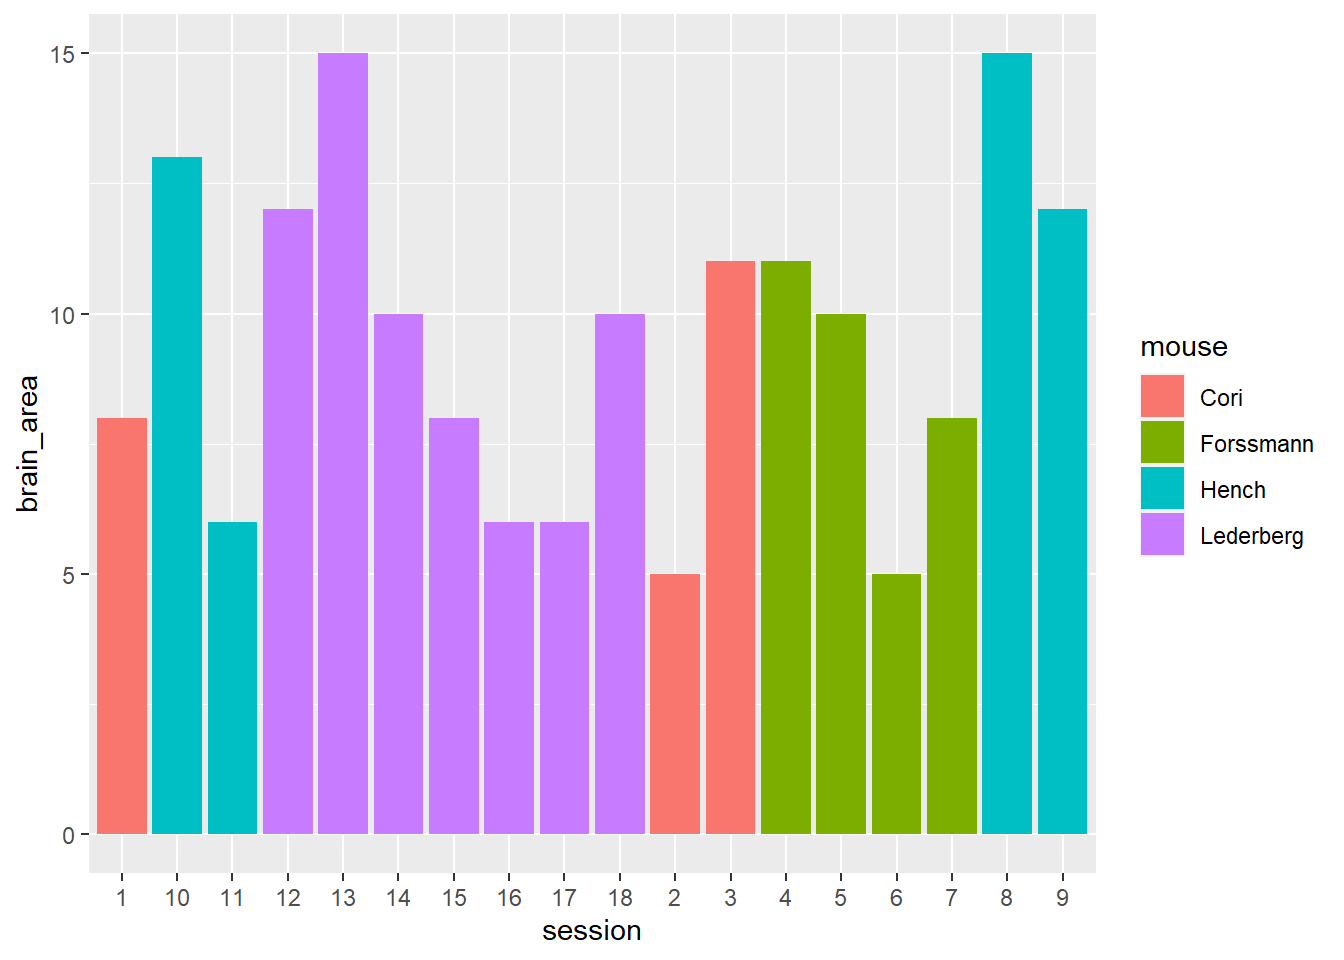
\includegraphics{images/unnamed-chunk-3-1.png}

\textbf{Manipulate Data Function}

Creating a function that aggregates the spike data in sessions and
stores them into a data frame

The ``manipulateData'' function is designed to aggregate the spike data
within each session and store it in a data frame. It takes a list
(referred to as session{[}i{]}) as input and extracts the spike data
while summing across the rows, excluding the time bin factor.

\begin{Shaded}
\begin{Highlighting}[]
\DocumentationTok{\#\#Takes an input of a list (AKA session[[i]]), and extracts out the spike data  and sums across the rows, excluding the time bin factor.}
\NormalTok{manipulateData}\OtherTok{\textless{}{-}}\ControlFlowTok{function}\NormalTok{(data,sessionNum)\{}
  
  
  \CommentTok{\#Number of trials for each session}
\NormalTok{  trial\_nums }\OtherTok{=} \ConstantTok{NULL}
  
  \CommentTok{\#Allocating variables}
\NormalTok{  brain\_area}\OtherTok{\textless{}{-}}\NormalTok{data}\SpecialCharTok{$}\NormalTok{brain\_area}
\NormalTok{  spks}\OtherTok{\textless{}{-}}\FunctionTok{cbind}\NormalTok{(brain\_area,}\FunctionTok{as.data.frame}\NormalTok{(}\FunctionTok{sapply}\NormalTok{(data}\SpecialCharTok{$}\NormalTok{spks,rowSums)))}
\NormalTok{  spks}\OtherTok{\textless{}{-}}\NormalTok{spks }\SpecialCharTok{\%\textgreater{}\%} \FunctionTok{group\_by}\NormalTok{(brain\_area) }\SpecialCharTok{\%\textgreater{}\%} \FunctionTok{summarise}\NormalTok{(}\FunctionTok{across}\NormalTok{(}\FunctionTok{everything}\NormalTok{(), sum))}
  
  
  \CommentTok{\#Pivoting the data frame}
\NormalTok{  proper }\OtherTok{\textless{}{-}}\NormalTok{ tidyr}\SpecialCharTok{::}\FunctionTok{pivot\_longer}\NormalTok{(spks, }\AttributeTok{cols =} \FunctionTok{starts\_with}\NormalTok{(}\StringTok{"V"}\NormalTok{), }\AttributeTok{names\_to =} \StringTok{"Trial"}\NormalTok{, }\AttributeTok{values\_to =} \StringTok{"Spikes"}\NormalTok{)}


  
\NormalTok{trial\_numbers }\OtherTok{\textless{}{-}} \FunctionTok{as.numeric}\NormalTok{(}\FunctionTok{sub}\NormalTok{(}\StringTok{"V"}\NormalTok{, }\StringTok{""}\NormalTok{, }\FunctionTok{grep}\NormalTok{(}\StringTok{"\^{}V}\SpecialCharTok{\textbackslash{}\textbackslash{}}\StringTok{d+$"}\NormalTok{, }\FunctionTok{names}\NormalTok{(spks), }\AttributeTok{value =} \ConstantTok{TRUE}\NormalTok{)))}

\CommentTok{\# Get the column names starting with "V" and extract the numeric part}
\NormalTok{trial\_nums}\OtherTok{\textless{}{-}}\FunctionTok{rep}\NormalTok{(trial\_numbers,}\FunctionTok{dim}\NormalTok{(proper }\SpecialCharTok{\%\textgreater{}\%} \FunctionTok{distinct}\NormalTok{(brain\_area))[}\DecValTok{1}\NormalTok{])}
\NormalTok{proper}\SpecialCharTok{$}\NormalTok{Trial}\OtherTok{\textless{}{-}}\FunctionTok{c}\NormalTok{(trial\_nums)}




\NormalTok{proper}\SpecialCharTok{$}\NormalTok{session}\OtherTok{\textless{}{-}}\NormalTok{sessionNum}

\FunctionTok{return}\NormalTok{(proper)}
  
\NormalTok{\}}
\end{Highlighting}
\end{Shaded}

\textbf{Creating the data frame for spikes}

\begin{Shaded}
\begin{Highlighting}[]
\CommentTok{\#Allocating the spike data frame}
\NormalTok{totalSpikeData}\OtherTok{\textless{}{-}}\ConstantTok{NULL}

\ControlFlowTok{for}\NormalTok{(i }\ControlFlowTok{in} \DecValTok{1}\SpecialCharTok{:}\DecValTok{18}\NormalTok{)\{}
  
  \CommentTok{\#Place holder for the spike data}
\NormalTok{  tempData }\OtherTok{\textless{}{-}}\FunctionTok{manipulateData}\NormalTok{(session[[i]],i)}
  
  
  \CommentTok{\#binding it to the data frame}
\NormalTok{  totalSpikeData}\OtherTok{\textless{}{-}} \FunctionTok{rbind}\NormalTok{(totalSpikeData,tempData)}
\NormalTok{\}}


\CommentTok{\#Checking dimensions}
\FunctionTok{dim}\NormalTok{(totalSpikeData)}
\end{Highlighting}
\end{Shaded}

\begin{verbatim}
## [1] 49173     4
\end{verbatim}

\begin{Shaded}
\begin{Highlighting}[]
\CommentTok{\#Confirming number of rows is correct for the newly created data frame}
\FunctionTok{sum}\NormalTok{((mouseData }\SpecialCharTok{\%\textgreater{}\%} \FunctionTok{distinct}\NormalTok{(brain\_area,number\_of\_trials)}\SpecialCharTok{\%\textgreater{}\%} \FunctionTok{pull}\NormalTok{(brain\_area) }\SpecialCharTok{\%\textgreater{}\%} \FunctionTok{as.numeric}\NormalTok{())}\SpecialCharTok{*}\NormalTok{ (mouseData }\SpecialCharTok{\%\textgreater{}\%} \FunctionTok{distinct}\NormalTok{(brain\_area,number\_of\_trials)}\SpecialCharTok{\%\textgreater{}\%} \FunctionTok{pull}\NormalTok{(number\_of\_trials) }\SpecialCharTok{\%\textgreater{}\%} \FunctionTok{as.numeric}\NormalTok{()))}
\end{Highlighting}
\end{Shaded}

\begin{verbatim}
## [1] 49173
\end{verbatim}

\textbf{Visualizations for spike activity per session}

By grouping the total number of spikes in each trial and visualizing the
data using a line graph, I can gain insights into the spike activity per
session. This approach allows us to understand the ranges and variations
in spike counts across the trials.

Upon examining the graph, I observe that some sessions have higher total
spike counts compared to others. This difference could be attributed to
factors such as the involvement of different mice or the application of
more neuron readers to specific brain areas within the cortex. However,
our main focus is on identifying differences in trends and fluctuations.
Upon closer examination, I notice that some mice experience fatigue,
leading to fluctuations in their total spike counts, while others
maintain a more consistent average.

Despite the variations, I can observe that there are similarities in
spike trends across sessions, suggesting common underlying patterns or
dynamics in the neural activity.

\begin{Shaded}
\begin{Highlighting}[]
\CommentTok{\#Session numbers for a random sampling method (removing bias)}
\NormalTok{sessionNumbers}\OtherTok{\textless{}{-}}\DecValTok{1}\SpecialCharTok{:}\DecValTok{18}


\DocumentationTok{\#\#Selecting Random sessions to plot and see association between number of spikes and Trial number}
\ControlFlowTok{for}\NormalTok{(i }\ControlFlowTok{in} \FunctionTok{sample}\NormalTok{(sessionNumbers,}\DecValTok{6}\NormalTok{,}\AttributeTok{replace =}\NormalTok{ F))\{}

\FunctionTok{print}\NormalTok{(}\FunctionTok{ggplot}\NormalTok{(totalSpikeData }\SpecialCharTok{\%\textgreater{}\%} \FunctionTok{filter}\NormalTok{(session }\SpecialCharTok{==}\NormalTok{ i) }\SpecialCharTok{\%\textgreater{}\%} \FunctionTok{group\_by}\NormalTok{(Trial) }\SpecialCharTok{\%\textgreater{}\%} \FunctionTok{summarise}\NormalTok{(}\AttributeTok{AverageSpikes =} \FunctionTok{mean}\NormalTok{(Spikes),}\AttributeTok{TotalSpikes =} \FunctionTok{sum}\NormalTok{(Spikes),}\AttributeTok{FiringRate =} \FunctionTok{sum}\NormalTok{(TotalSpikes)}\SpecialCharTok{/}\DecValTok{734}\NormalTok{),}\FunctionTok{aes}\NormalTok{(}\AttributeTok{x =}\NormalTok{ Trial,}\AttributeTok{y =}\NormalTok{ TotalSpikes))}\SpecialCharTok{+}\FunctionTok{geom\_line}\NormalTok{()}\SpecialCharTok{+}\FunctionTok{labs}\NormalTok{(}\AttributeTok{y =} \StringTok{"Total Number of Spikes"}\NormalTok{,}\AttributeTok{x =} \StringTok{"Trial Number"}\NormalTok{,}\AttributeTok{title =} \FunctionTok{paste}\NormalTok{(}\StringTok{"session"}\NormalTok{,i)))}
\NormalTok{\}}
\end{Highlighting}
\end{Shaded}

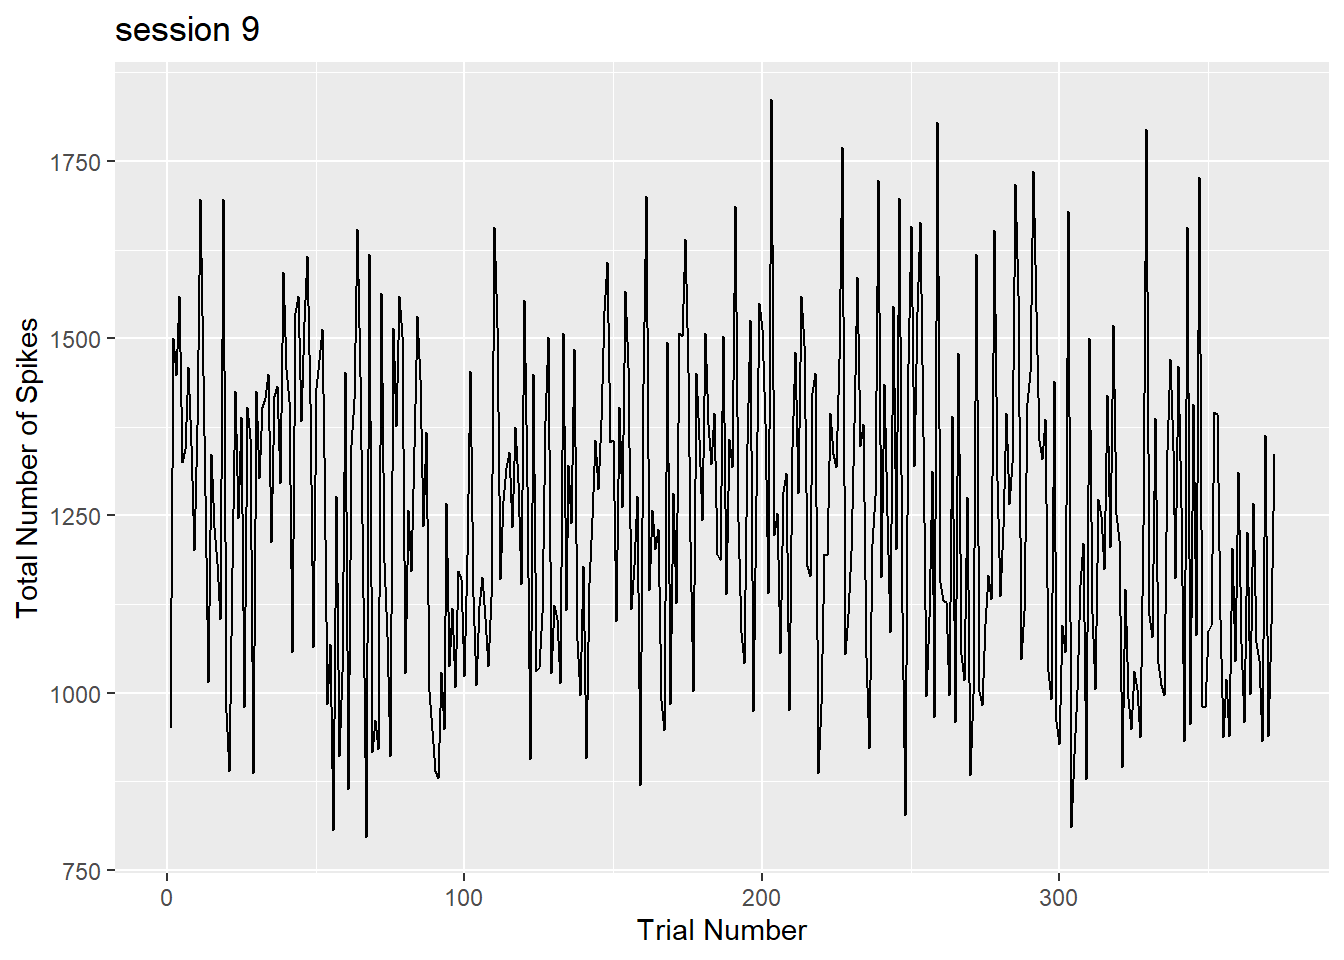
\includegraphics{images/unnamed-chunk-6-1.png}
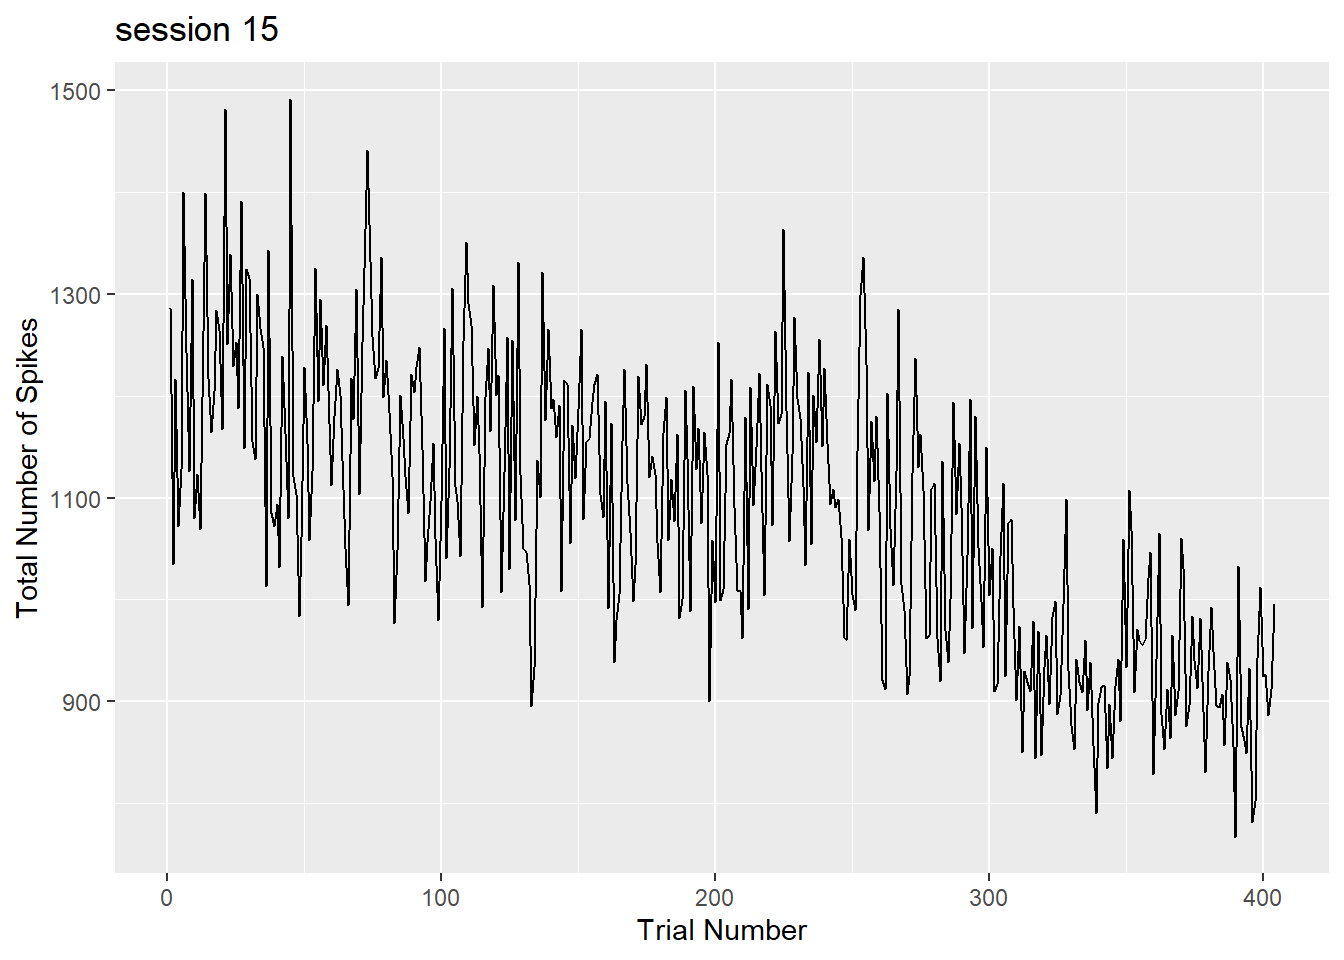
\includegraphics{images/unnamed-chunk-6-2.png}
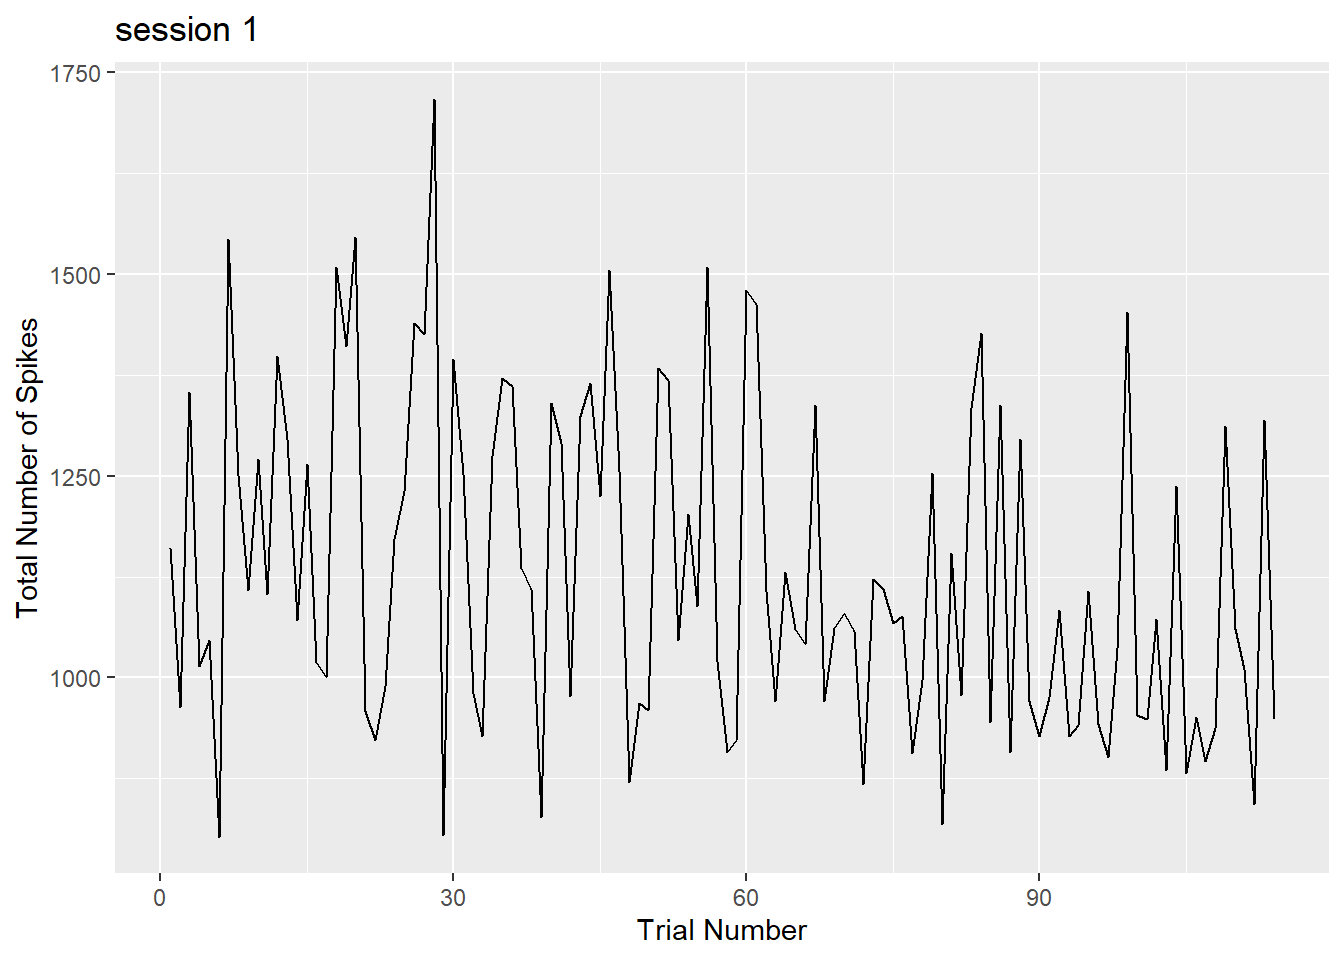
\includegraphics{images/unnamed-chunk-6-3.png}
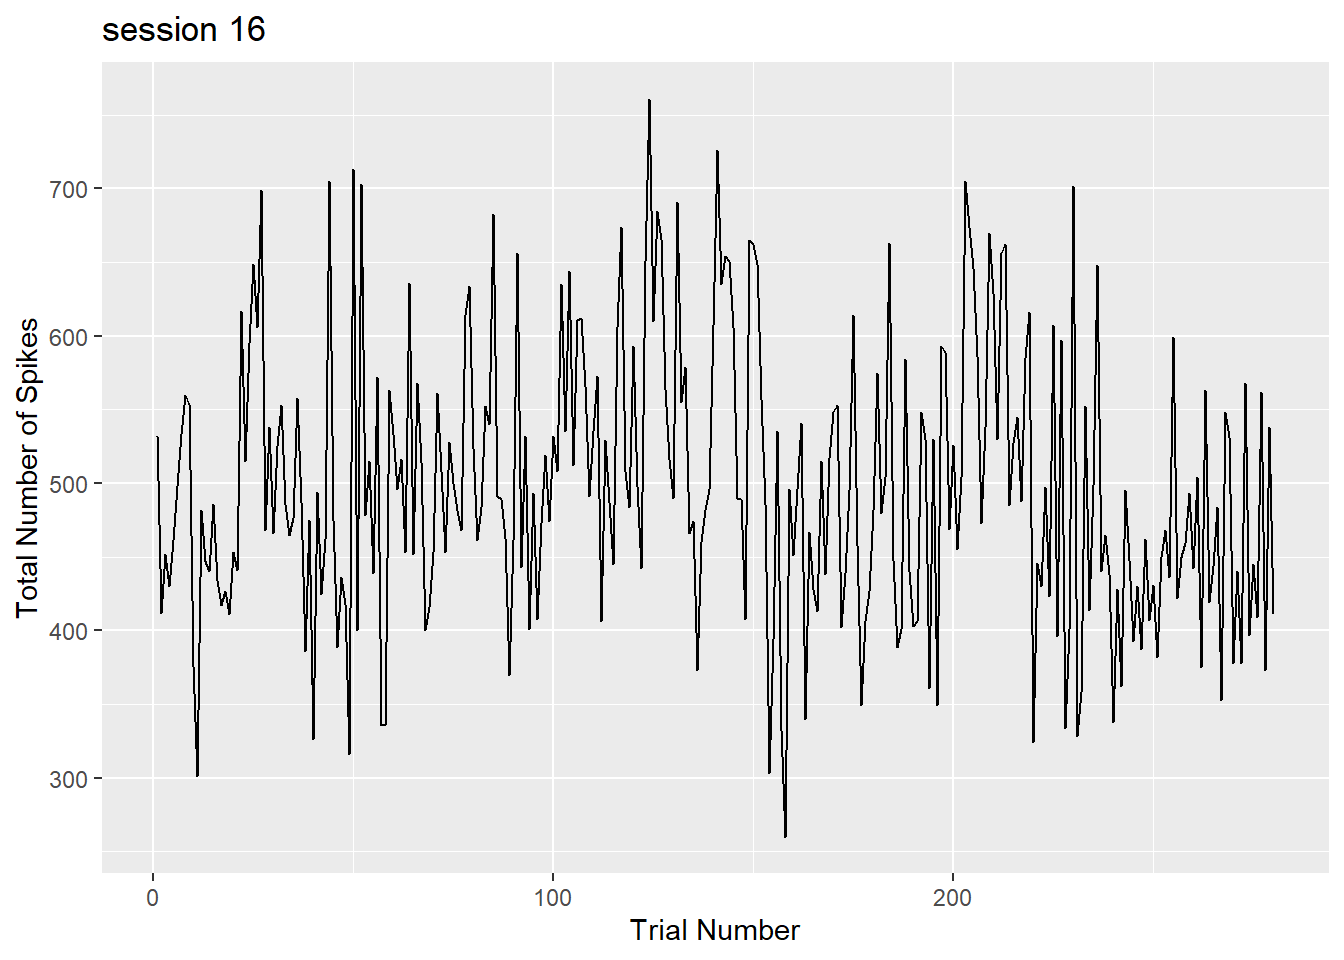
\includegraphics{images/unnamed-chunk-6-4.png}
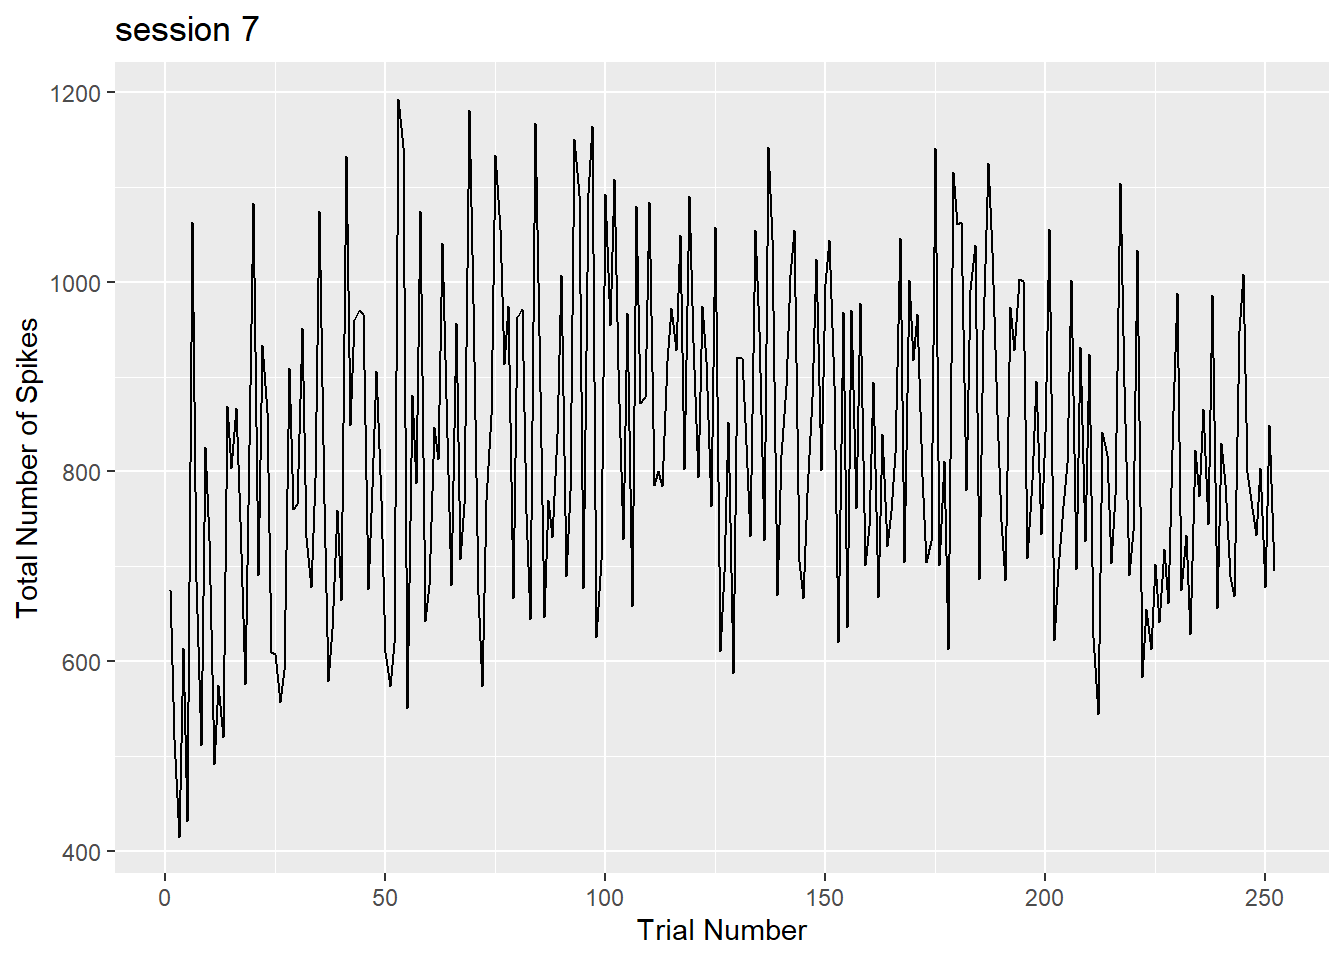
\includegraphics{images/unnamed-chunk-6-5.png}
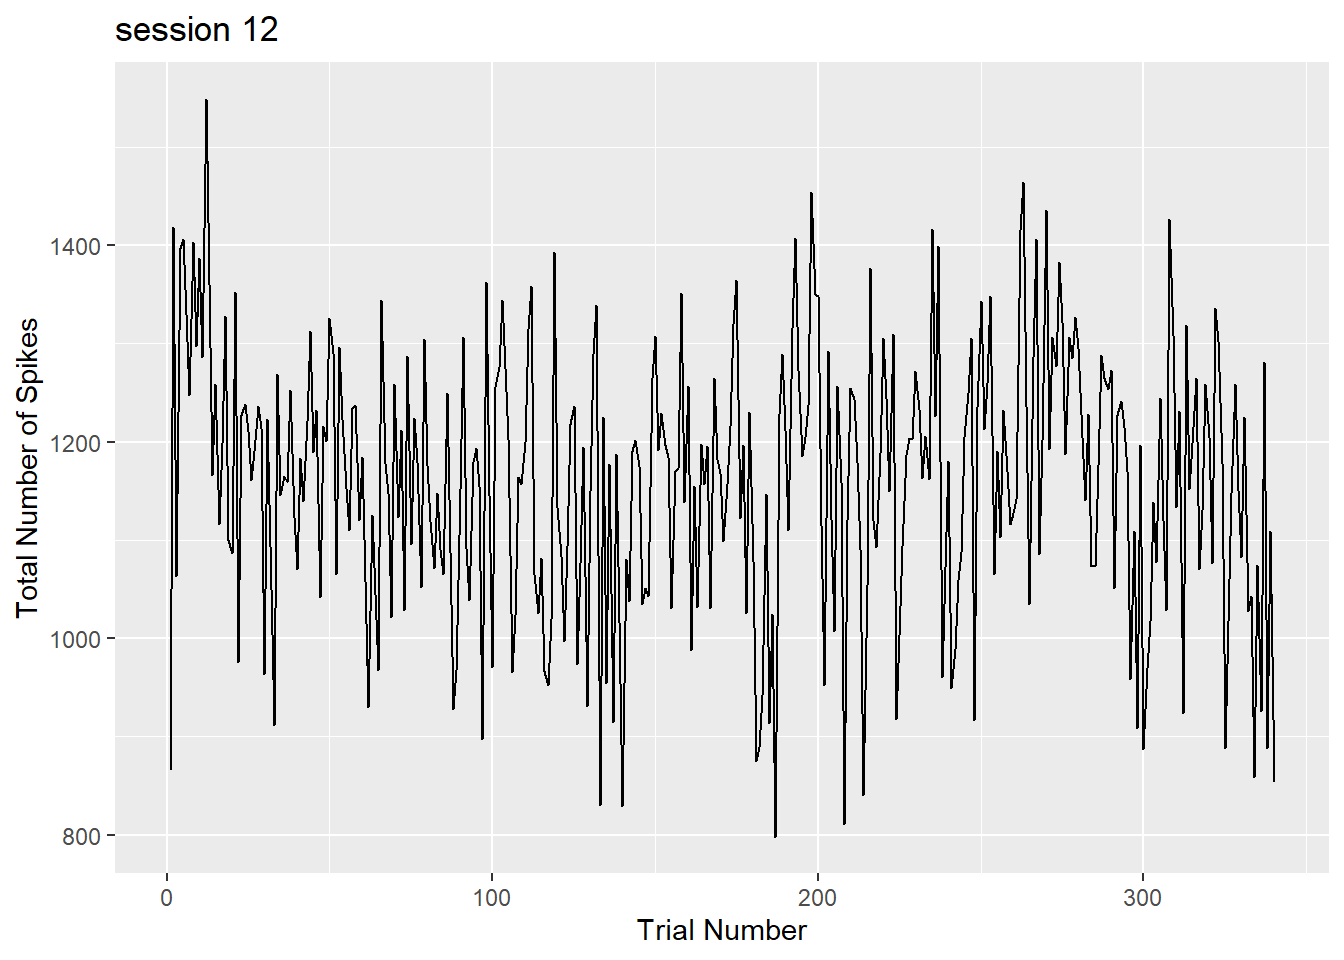
\includegraphics{images/unnamed-chunk-6-6.png}

\textbf{Analyzing Spike Activity Across Different Brain Areas}

To explore the spike activity per brain area, I select arbitrary
sessions to analyze the trends. This approach helps eliminate bias and
allows us to observe patterns in neural activity across different brain
areas.

By examining the spike activity in these sessions, I can identify how
neurons in specific brain areas respond to the stimuli presented during
the trials. This analysis provides insights into the functional
properties and information processing capabilities of different regions
within the visual cortex.

By considering multiple sessions and brain areas, I can gain a more
comprehensive understanding of the neural dynamics and potentially
uncover common patterns or variations in spike activity across different
experimental conditions.

\begin{Shaded}
\begin{Highlighting}[]
\ControlFlowTok{for}\NormalTok{(i }\ControlFlowTok{in} \FunctionTok{sample}\NormalTok{(sessionNumbers,}\DecValTok{5}\NormalTok{,}\AttributeTok{replace =}\NormalTok{ F))\{}
  
  \FunctionTok{print}\NormalTok{(}\FunctionTok{ggplot}\NormalTok{(totalSpikeData }\SpecialCharTok{\%\textgreater{}\%} \FunctionTok{filter}\NormalTok{(session }\SpecialCharTok{==}\NormalTok{ i),}\FunctionTok{aes}\NormalTok{(}\AttributeTok{x =}\NormalTok{ Trial,}\AttributeTok{y =}\NormalTok{ Spikes,}\AttributeTok{color =}\NormalTok{ brain\_area))}\SpecialCharTok{+} \FunctionTok{geom\_line}\NormalTok{()}\SpecialCharTok{+}\FunctionTok{labs}\NormalTok{(}\AttributeTok{y =} \StringTok{"Total Number of Spikes Per Brain Area"}\NormalTok{,}\AttributeTok{x =} \StringTok{"Trial Number"}\NormalTok{,}\AttributeTok{title =} \FunctionTok{paste}\NormalTok{(}\StringTok{"session"}\NormalTok{,i)))}

  
\NormalTok{\}}
\end{Highlighting}
\end{Shaded}

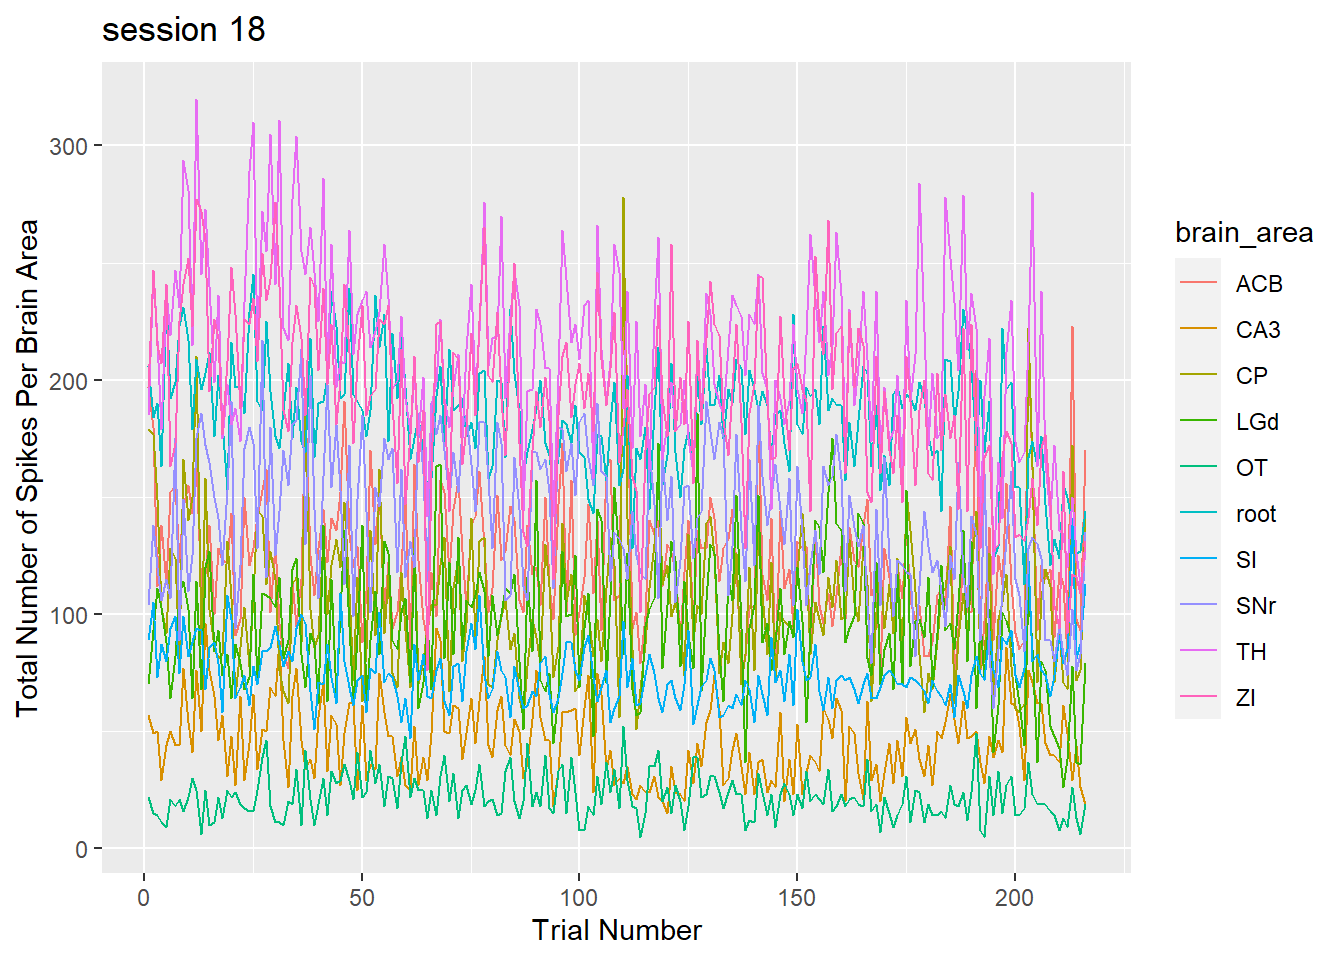
\includegraphics{images/unnamed-chunk-7-1.png}
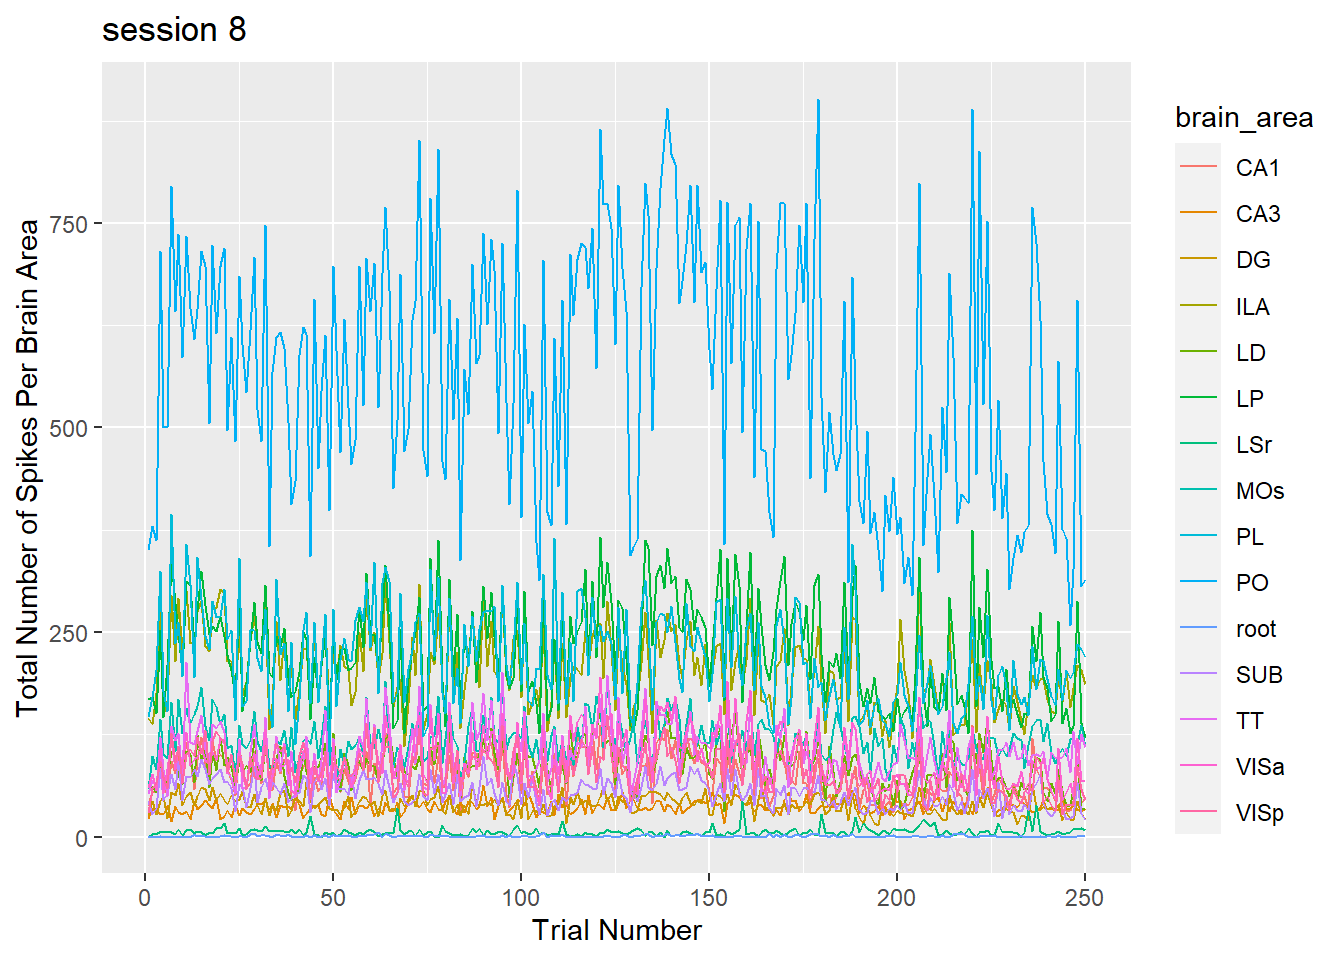
\includegraphics{images/unnamed-chunk-7-2.png}
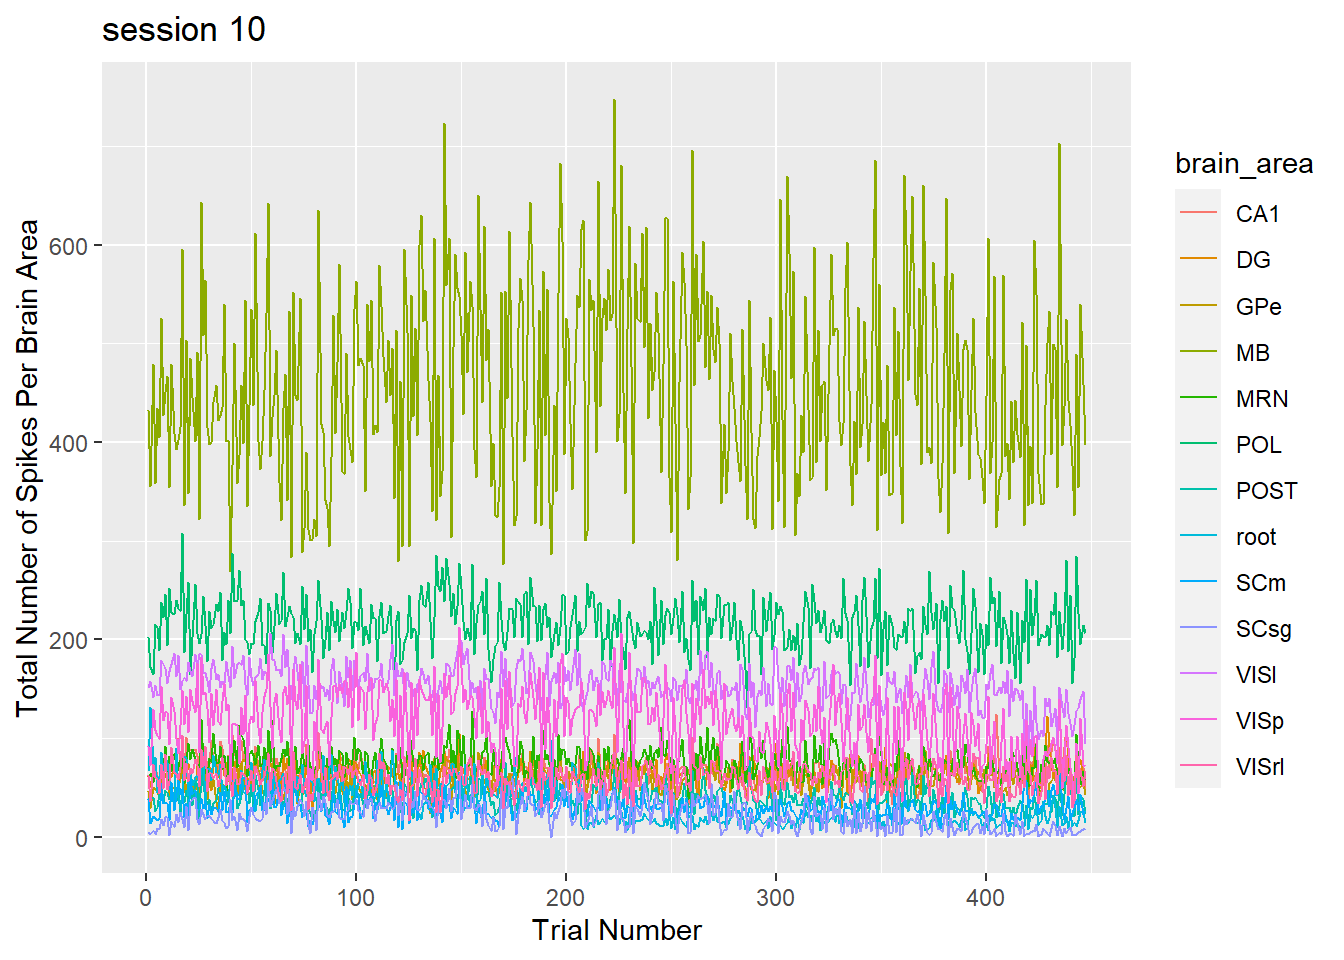
\includegraphics{images/unnamed-chunk-7-3.png}
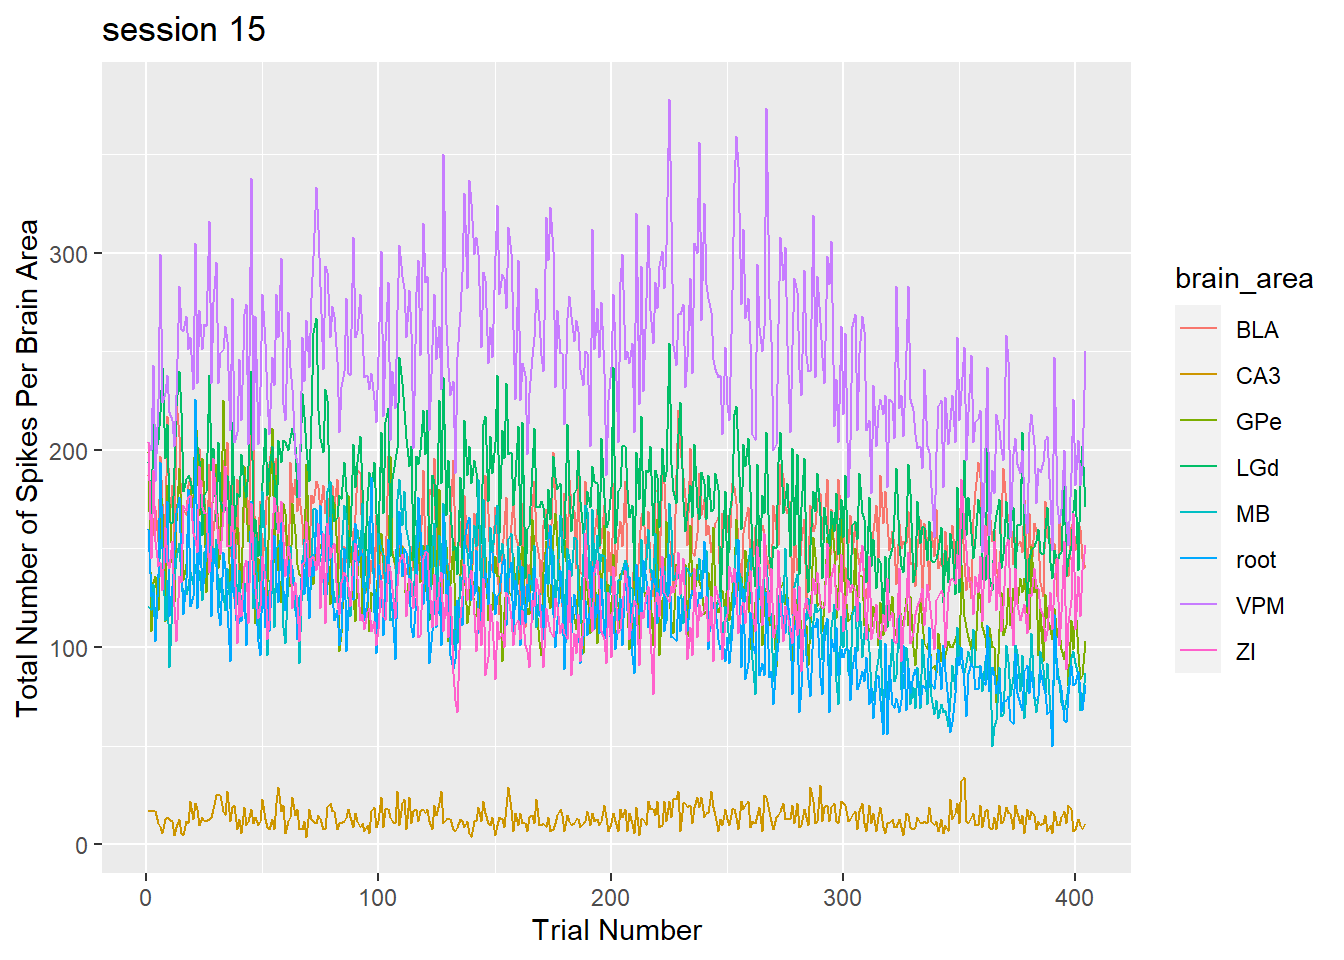
\includegraphics{images/unnamed-chunk-7-4.png}
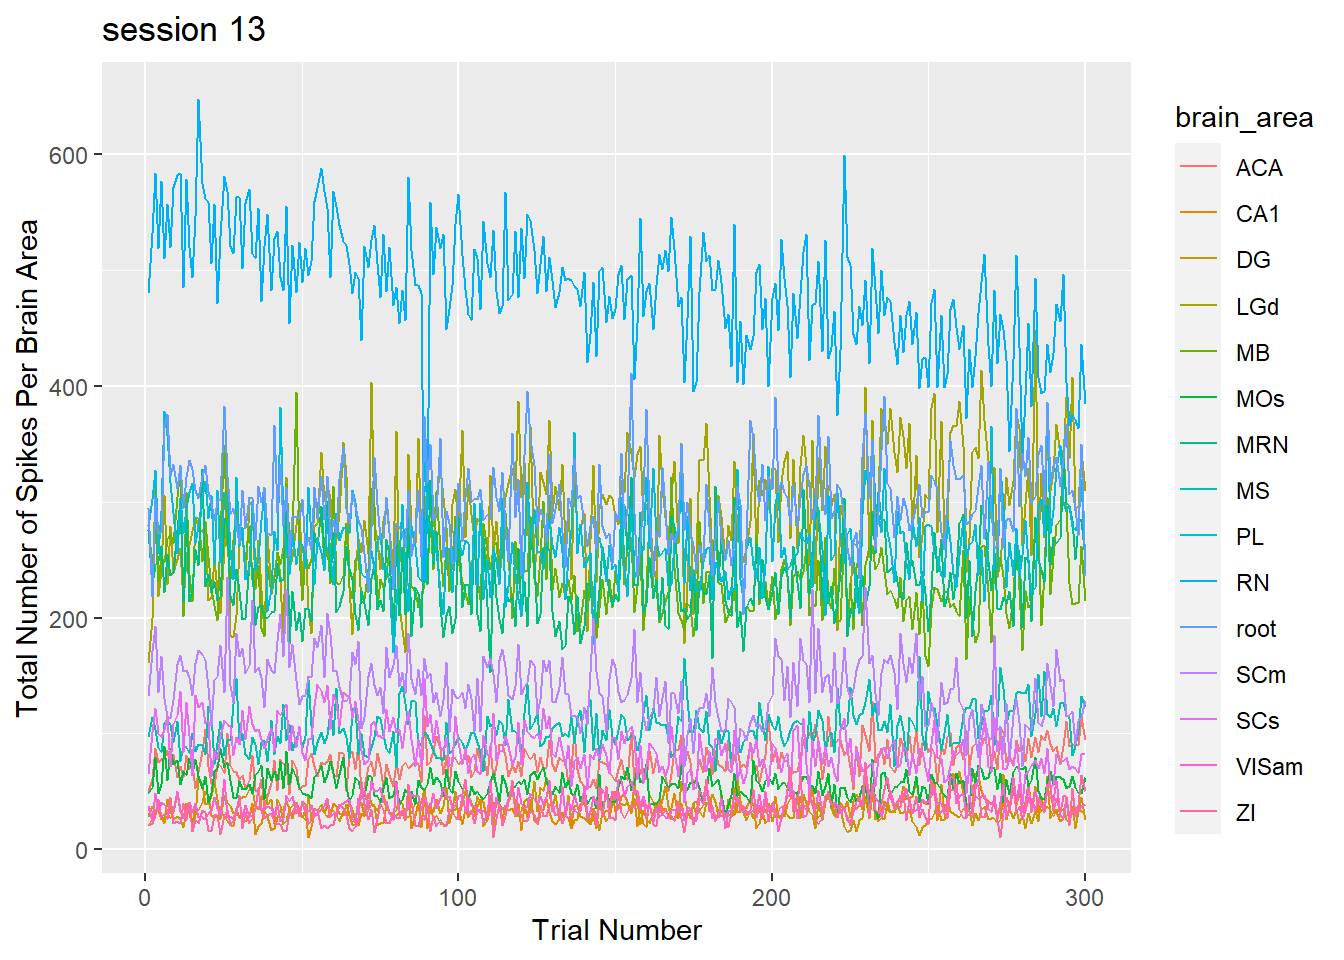
\includegraphics{images/unnamed-chunk-7-5.png}

\section{Data Integration}\label{data-integration}

In the Data Integration phase, I leverage the insights gained from Part
1 to develop an approach for combining data across trials. The main
objective is to extract shared patterns across sessions and address the
differences between sessions, enabling us to borrow information and
improve the prediction performance in Part 3.

To achieve this, I employ two strategies:

Extracting Shared Patterns: I identify common patterns and trends that
exist across multiple sessions. By identifying these shared features, I
can capture the underlying patterns that contribute to the neural
activity during trials.

Addressing Session Differences: I take into account the variations
between sessions, such as differences in brain areas or spike activity,
feedback type, etc. By addressing these session-specific factors, I can
account for potential biases and ensure a more robust and accurate
prediction model.

\textbf{I will now perform some data manipulation in order to combine
the spike data with the mouse data}

\begin{Shaded}
\begin{Highlighting}[]
\DocumentationTok{\#\#Summarizing the spike data in order to merge it with the mouse data}
\NormalTok{summarisedSpikeData}\OtherTok{\textless{}{-}}\NormalTok{ totalSpikeData }\SpecialCharTok{\%\textgreater{}\%}  \FunctionTok{group\_by}\NormalTok{(session,Trial) }\SpecialCharTok{\%\textgreater{}\%} \FunctionTok{summarise}\NormalTok{(}\AttributeTok{spikes =} \FunctionTok{sum}\NormalTok{(Spikes))}
\end{Highlighting}
\end{Shaded}

\begin{verbatim}
## `summarise()` has grouped output by 'session'. You can override using the
## `.groups` argument.
\end{verbatim}

\begin{Shaded}
\begin{Highlighting}[]
\NormalTok{perfectMouseData}\OtherTok{\textless{}{-}}\FunctionTok{cbind}\NormalTok{(mouseData,summarisedSpikeData[}\SpecialCharTok{{-}}\DecValTok{1}\NormalTok{])}



\DocumentationTok{\#\#Creating the perfect mouse data.}
\FunctionTok{head}\NormalTok{(perfectMouseData,}\DecValTok{20}\NormalTok{)}
\end{Highlighting}
\end{Shaded}

\begin{verbatim}
##    contrast_left contrast_right session mouse number_of_neurons brain_area
## 1              0            0.5       1  Cori               734          8
## 2              0              0       1  Cori               734          8
## 3            0.5              1       1  Cori               734          8
## 4              0              0       1  Cori               734          8
## 5              0              0       1  Cori               734          8
## 6              0              0       1  Cori               734          8
## 7              1            0.5       1  Cori               734          8
## 8            0.5              0       1  Cori               734          8
## 9              0              0       1  Cori               734          8
## 10           0.5           0.25       1  Cori               734          8
## 11           0.5              0       1  Cori               734          8
## 12             0              1       1  Cori               734          8
## 13             1              1       1  Cori               734          8
## 14             0              0       1  Cori               734          8
## 15             0              0       1  Cori               734          8
## 16             0              0       1  Cori               734          8
## 17             0              0       1  Cori               734          8
## 18             0            0.5       1  Cori               734          8
## 19           0.5           0.25       1  Cori               734          8
## 20          0.25              1       1  Cori               734          8
##    number_of_trials feedback_type Trial spikes
## 1               114             1     1   1161
## 2               114             1     2    963
## 3               114            -1     3   1354
## 4               114            -1     4   1014
## 5               114            -1     5   1046
## 6               114             1     6    803
## 7               114             1     7   1543
## 8               114             1     8   1251
## 9               114             1     9   1108
## 10              114             1    10   1271
## 11              114             1    11   1104
## 12              114             1    12   1398
## 13              114            -1    13   1295
## 14              114            -1    14   1071
## 15              114            -1    15   1265
## 16              114            -1    16   1019
## 17              114             1    17   1001
## 18              114             1    18   1508
## 19              114             1    19   1410
## 20              114             1    20   1545
\end{verbatim}

To analyze the distribution of feedback types (success or failure)
across sessions and identify any consistent patterns or trends, I
utilized bar charts. These charts visually represented the distribution
of feedback types across sessions, providing insights into the
relationship between sessions and feedback outcomes.

I generated two bar charts for this analysis. The first chart displayed
the absolute counts of success and failure without any scaling. This
allowed me to observe the raw differences in the total
success-to-failure ratio across sessions. By examining this chart, I
could identify sessions with notable variations in the distribution of
feedback types.

To gain a better understanding of the proportional differences between
sessions, I created a second bar chart with scaling. This chart allowed
me to compare the proportions of success and failure across sessions,
normalizing the data and enabling a more direct comparison. By
visualizing the scaled proportions, I could identify any consistent
patterns or trends in the distribution of feedback types across
sessions.

\subsection{Shared Patterns Across
Sessions}\label{shared-patterns-across-sessions}

\begin{Shaded}
\begin{Highlighting}[]
\DocumentationTok{\#\#Total counts data set}
\NormalTok{feedback\_counts }\OtherTok{\textless{}{-}}\NormalTok{ perfectMouseData }\SpecialCharTok{\%\textgreater{}\%}
  \FunctionTok{group\_by}\NormalTok{(session, feedback\_type) }\SpecialCharTok{\%\textgreater{}\%}
  \FunctionTok{summarise}\NormalTok{(}\AttributeTok{count =} \FunctionTok{n}\NormalTok{()) }\SpecialCharTok{\%\textgreater{}\%} \FunctionTok{group\_by}\NormalTok{(session) }\SpecialCharTok{\%\textgreater{}\%} \FunctionTok{mutate}\NormalTok{(}\AttributeTok{totals =} \FunctionTok{sum}\NormalTok{(count))}
\end{Highlighting}
\end{Shaded}

\begin{verbatim}
## `summarise()` has grouped output by 'session'. You can override using the
## `.groups` argument.
\end{verbatim}

\begin{Shaded}
\begin{Highlighting}[]
\CommentTok{\#Feedback proportions data set}
\NormalTok{feedback\_proportions }\OtherTok{\textless{}{-}}\NormalTok{ perfectMouseData }\SpecialCharTok{\%\textgreater{}\%}
  \FunctionTok{group\_by}\NormalTok{(session, feedback\_type) }\SpecialCharTok{\%\textgreater{}\%}
  \FunctionTok{summarise}\NormalTok{(}\AttributeTok{count =} \FunctionTok{n}\NormalTok{()) }\SpecialCharTok{\%\textgreater{}\%} \FunctionTok{mutate}\NormalTok{(}\AttributeTok{percentage =}\NormalTok{ count}\SpecialCharTok{/}\FunctionTok{sum}\NormalTok{(count))}
\end{Highlighting}
\end{Shaded}

\begin{verbatim}
## `summarise()` has grouped output by 'session'. You can override using the
## `.groups` argument.
\end{verbatim}

\begin{Shaded}
\begin{Highlighting}[]
\DocumentationTok{\#\#Total counts of feedback}
\NormalTok{total\_counts }\OtherTok{=}\NormalTok{ feedback\_counts }\SpecialCharTok{\%\textgreater{}\%} \FunctionTok{group\_by}\NormalTok{(session) }\SpecialCharTok{\%\textgreater{}\%} \FunctionTok{summarise}\NormalTok{(}\AttributeTok{total =} \FunctionTok{sum}\NormalTok{(count))}

\DocumentationTok{\#\#Average feedback for success}
\NormalTok{average\_rate }\OtherTok{\textless{}{-}}\NormalTok{ feedback\_proportions }\SpecialCharTok{\%\textgreater{}\%}\FunctionTok{filter}\NormalTok{(feedback\_type }\SpecialCharTok{==}\DecValTok{1}\NormalTok{) }\SpecialCharTok{\%\textgreater{}\%} \FunctionTok{pull}\NormalTok{(percentage) }\SpecialCharTok{\%\textgreater{}\%} \FunctionTok{mean}\NormalTok{()}



\NormalTok{feedback\_counts }
\end{Highlighting}
\end{Shaded}

\begin{verbatim}
## # A tibble: 36 x 4
## # Groups:   session [18]
##    session feedback_type count totals
##    <fct>   <fct>         <int>  <int>
##  1 1       -1               45    114
##  2 1       1                69    114
##  3 10      -1              170    447
##  4 10      1               277    447
##  5 11      -1               70    342
##  6 11      1               272    342
##  7 12      -1               89    340
##  8 12      1               251    340
##  9 13      -1               61    300
## 10 13      1               239    300
## # i 26 more rows
\end{verbatim}

\begin{Shaded}
\begin{Highlighting}[]
\FunctionTok{ggplot}\NormalTok{(feedback\_counts, }\FunctionTok{aes}\NormalTok{(}\AttributeTok{x =}\NormalTok{ session, }\AttributeTok{y =}\NormalTok{ count, }\AttributeTok{fill =}\NormalTok{ feedback\_type)) }\SpecialCharTok{+}
  \FunctionTok{geom\_bar}\NormalTok{(}\AttributeTok{stat =} \StringTok{"identity"}\NormalTok{) }\SpecialCharTok{+} \FunctionTok{geom\_text}\NormalTok{(}\FunctionTok{aes}\NormalTok{(}\AttributeTok{label =}\NormalTok{ totals),}\AttributeTok{vjust =} \SpecialCharTok{{-}}\NormalTok{.}\DecValTok{5}\NormalTok{,}\AttributeTok{color =} \StringTok{"black"}\NormalTok{)}\SpecialCharTok{+} \FunctionTok{scale\_fill\_manual}\NormalTok{(}\AttributeTok{values =} \FunctionTok{c}\NormalTok{(}\StringTok{"1"} \OtherTok{=} \StringTok{"black"}\NormalTok{, }\StringTok{"{-}1"} \OtherTok{=} \StringTok{"red"}\NormalTok{)) }\SpecialCharTok{+} \FunctionTok{labs}\NormalTok{(}\AttributeTok{x =} \StringTok{"Session"}\NormalTok{, }\AttributeTok{y =} \StringTok{"Count"}\NormalTok{, }\AttributeTok{fill =} \StringTok{"Feedback Type"}\NormalTok{) }\SpecialCharTok{+} \FunctionTok{ggtitle}\NormalTok{(}\StringTok{"Distribution of Feedback Types Across Sessions"}\NormalTok{)}
\end{Highlighting}
\end{Shaded}

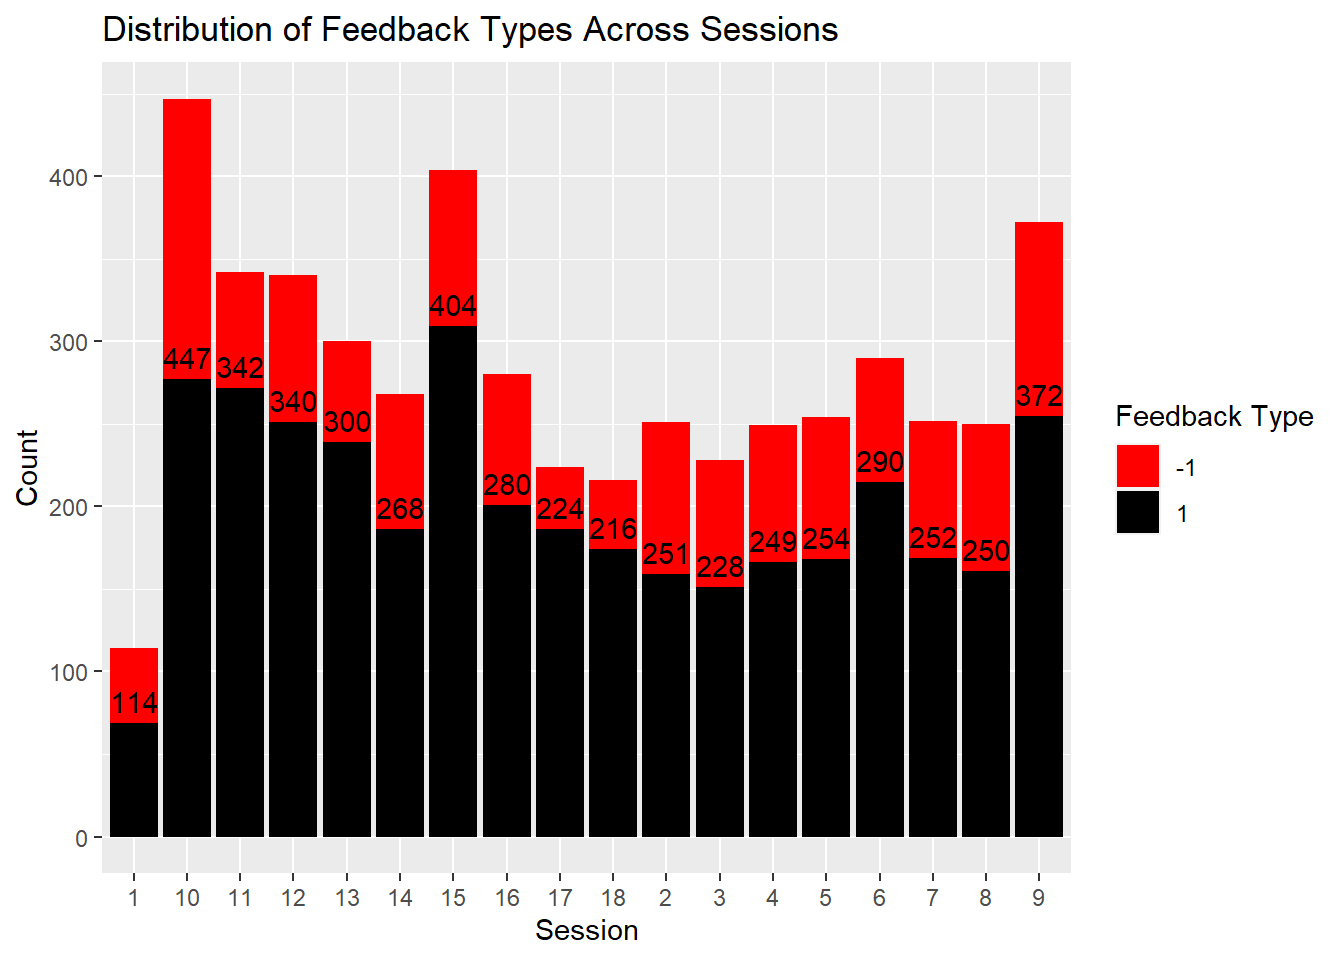
\includegraphics{images/unnamed-chunk-9-1.png}

\begin{Shaded}
\begin{Highlighting}[]
\FunctionTok{ggplot}\NormalTok{(feedback\_proportions, }\FunctionTok{aes}\NormalTok{(}\AttributeTok{x =}\NormalTok{ session, }\AttributeTok{y =}\NormalTok{ percentage, }\AttributeTok{fill =}\NormalTok{ feedback\_type)) }\SpecialCharTok{+}
  \FunctionTok{geom\_bar}\NormalTok{(}\AttributeTok{stat =} \StringTok{"identity"}\NormalTok{) }\SpecialCharTok{+}
  \FunctionTok{scale\_fill\_manual}\NormalTok{(}\AttributeTok{values =} \FunctionTok{c}\NormalTok{(}\StringTok{"1"} \OtherTok{=} \StringTok{"black"}\NormalTok{, }\StringTok{"{-}1"} \OtherTok{=} \StringTok{"red"}\NormalTok{)) }\SpecialCharTok{+} \FunctionTok{geom\_hline}\NormalTok{(}\AttributeTok{yintercept =}\NormalTok{ average\_rate, }\AttributeTok{linetype =} \StringTok{"dashed"}\NormalTok{, }\AttributeTok{color =} \StringTok{"yellow"}\NormalTok{,}\AttributeTok{size =}\NormalTok{ .}\DecValTok{7}\NormalTok{)}\SpecialCharTok{+}
  \FunctionTok{labs}\NormalTok{(}\AttributeTok{x =} \StringTok{"Session"}\NormalTok{, }\AttributeTok{y =} \StringTok{"Count"}\NormalTok{, }\AttributeTok{fill =} \StringTok{"Feedback Type"}\NormalTok{) }\SpecialCharTok{+}
  \FunctionTok{ggtitle}\NormalTok{(}\StringTok{"Distribution of Feedbacks Across Sessions"}\NormalTok{)}
\end{Highlighting}
\end{Shaded}

\begin{verbatim}
## Warning: Using `size` aesthetic for lines was deprecated in ggplot2 3.4.0.
## i Please use `linewidth` instead.
## This warning is displayed once every 8 hours.
## Call `lifecycle::last_lifecycle_warnings()` to see where this warning was
## generated.
\end{verbatim}

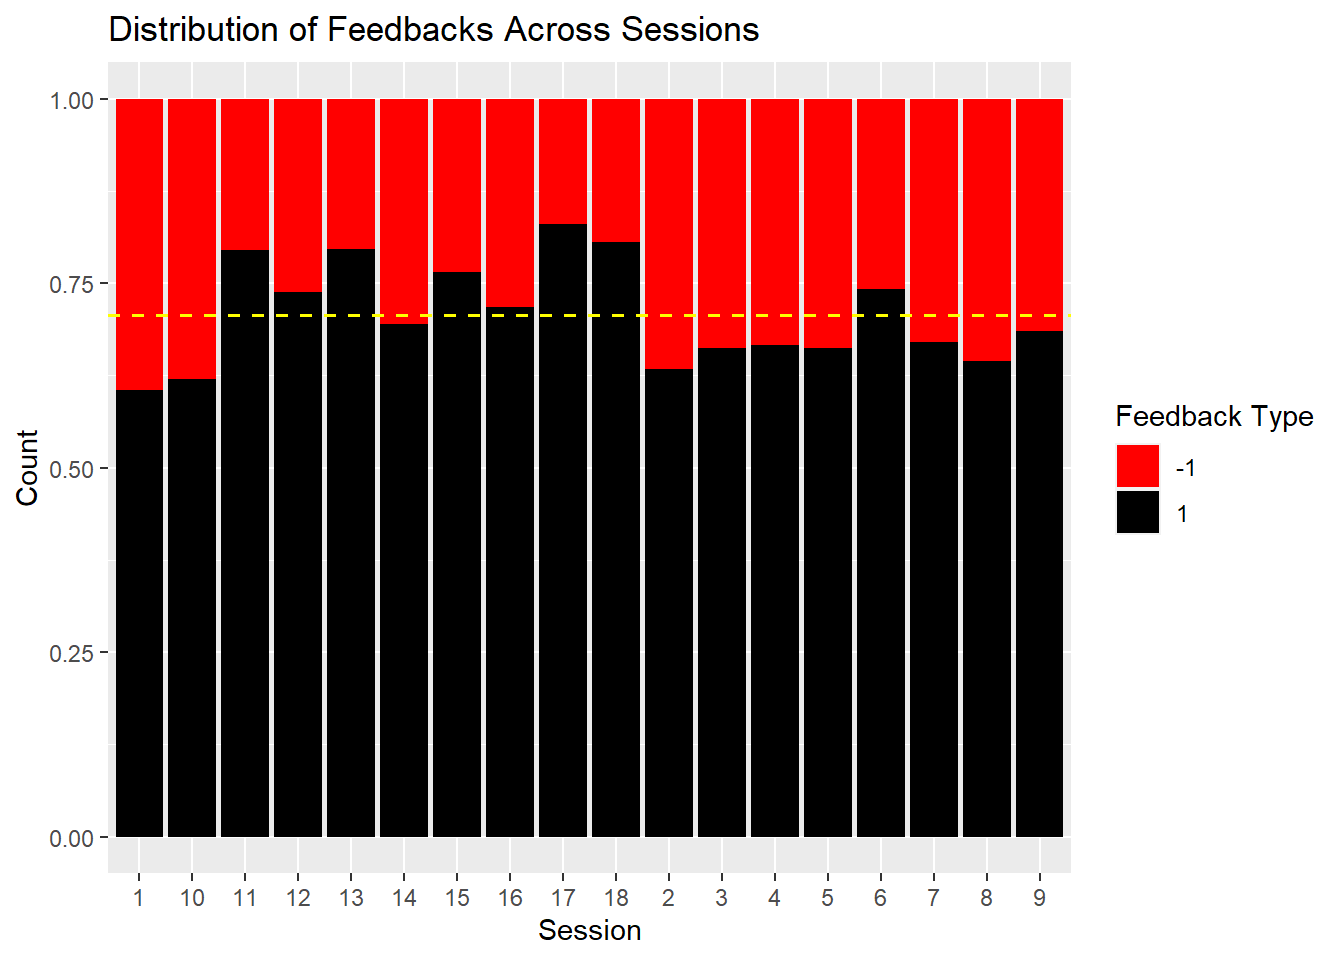
\includegraphics{images/unnamed-chunk-9-2.png}

\textbf{Exploring the Relationship Between Contrast Levels and Feedback
Type}

In this analysis, I delve into the relationship between the contrast
levels (contrast\_left and contrast\_right) and the feedback type across
sessions. Our aim is to investigate whether certain combinations of
contrast levels consistently result in success or failure.

By examining the data from various sessions, I can identify patterns and
trends that shed light on the influence of contrast levels on the
feedback outcomes. Specifically, I assess how different combinations of
contrast levels are associated with the feedback types, which are
categorized as success (1) or failure (-1).

This exploration provides valuable insights into the relationship
between visual stimuli (represented by contrast levels) and the
resulting feedback. By understanding the consistent associations between
specific contrast combinations and success/failure outcomes, I can gain
a deeper understanding of the decision-making process of the mice during
the trials.

Upon analyzing the data, I observe a significant portion of trials with
contrast levels of (0, 0), indicating the absence of visual stimuli.
Within this contrast level, I notice a higher occurrence of success
feedback compared to failures. This finding suggests that the mice
demonstrate an understanding of the absence of stimuli and refrain from
moving the wheel, resulting in successful outcomes. Other contrast
levels seem to be distributed fairly.

\begin{Shaded}
\begin{Highlighting}[]
\DocumentationTok{\#\#Distribution of contrast varieties across all sessions}
\NormalTok{contrastLevels }\OtherTok{\textless{}{-}}\NormalTok{  perfectMouseData }\SpecialCharTok{\%\textgreater{}\%} \FunctionTok{group\_by}\NormalTok{(contrast\_left,contrast\_right) }\SpecialCharTok{\%\textgreater{}\%} \FunctionTok{summarize}\NormalTok{(}\AttributeTok{counts =} \FunctionTok{n}\NormalTok{()) }
\end{Highlighting}
\end{Shaded}

\begin{verbatim}
## `summarise()` has grouped output by 'contrast_left'. You can override using the
## `.groups` argument.
\end{verbatim}

\begin{Shaded}
\begin{Highlighting}[]
\DocumentationTok{\#\#Distribution of contrast varieties across all sessions with feedback}
\NormalTok{contrastLevelsByFeedback }\OtherTok{=}\NormalTok{ perfectMouseData }\SpecialCharTok{\%\textgreater{}\%} \FunctionTok{group\_by}\NormalTok{(contrast\_left,contrast\_right,feedback\_type) }\SpecialCharTok{\%\textgreater{}\%} \FunctionTok{summarize}\NormalTok{(}\AttributeTok{counts =} \FunctionTok{n}\NormalTok{()) }
\end{Highlighting}
\end{Shaded}

\begin{verbatim}
## `summarise()` has grouped output by 'contrast_left', 'contrast_right'. You can
## override using the `.groups` argument.
\end{verbatim}

\begin{Shaded}
\begin{Highlighting}[]
\DocumentationTok{\#\#Plots}

\DocumentationTok{\#\#Counts of various Contrast Levels for trials}
\FunctionTok{ggplot}\NormalTok{(contrastLevels, }\FunctionTok{aes}\NormalTok{(}\AttributeTok{x =}\NormalTok{ contrast\_left, }\AttributeTok{y =}\NormalTok{ contrast\_right,}\AttributeTok{size =}\NormalTok{ counts}\SpecialCharTok{/}\DecValTok{100}\NormalTok{,}\AttributeTok{label =}\NormalTok{ counts)) }\SpecialCharTok{+}
  \FunctionTok{geom\_point}\NormalTok{()}\SpecialCharTok{+}\FunctionTok{geom\_text}\NormalTok{(}\AttributeTok{size =} \DecValTok{3}\NormalTok{, }\AttributeTok{vjust =} \SpecialCharTok{{-}}\FloatTok{1.2}\NormalTok{)}
\end{Highlighting}
\end{Shaded}

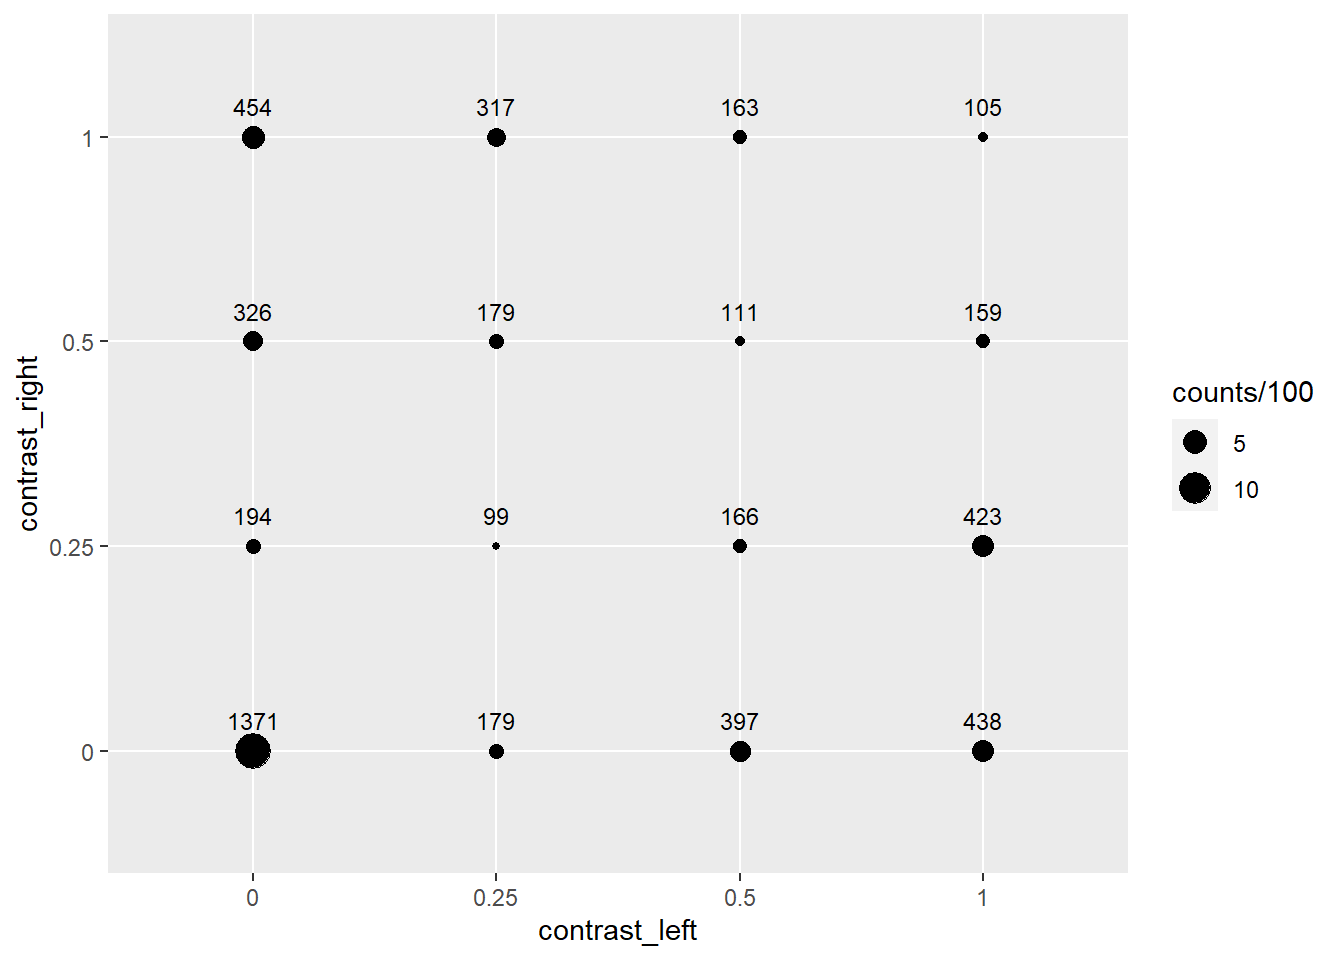
\includegraphics{images/unnamed-chunk-10-1.png}

\begin{Shaded}
\begin{Highlighting}[]
\DocumentationTok{\#\# Counts of trials depending on Contrast Levels faceted by feedback type}
\FunctionTok{ggplot}\NormalTok{(contrastLevelsByFeedback, }\FunctionTok{aes}\NormalTok{(}\AttributeTok{x =}\NormalTok{ contrast\_left, }\AttributeTok{y =}\NormalTok{ contrast\_right,}\AttributeTok{size =}\NormalTok{ counts}\SpecialCharTok{/}\DecValTok{100}\NormalTok{,}\AttributeTok{label =}\NormalTok{ counts,}\AttributeTok{color =}\NormalTok{ feedback\_type)) }\SpecialCharTok{+}
  \FunctionTok{geom\_point}\NormalTok{()}\SpecialCharTok{+}\FunctionTok{geom\_text}\NormalTok{(}\AttributeTok{size =} \DecValTok{3}\NormalTok{, }\AttributeTok{vjust =} \SpecialCharTok{{-}}\FloatTok{1.2}\NormalTok{)}\SpecialCharTok{+}\FunctionTok{facet\_grid}\NormalTok{(}\SpecialCharTok{\textasciitilde{}}\NormalTok{feedback\_type)}
\end{Highlighting}
\end{Shaded}

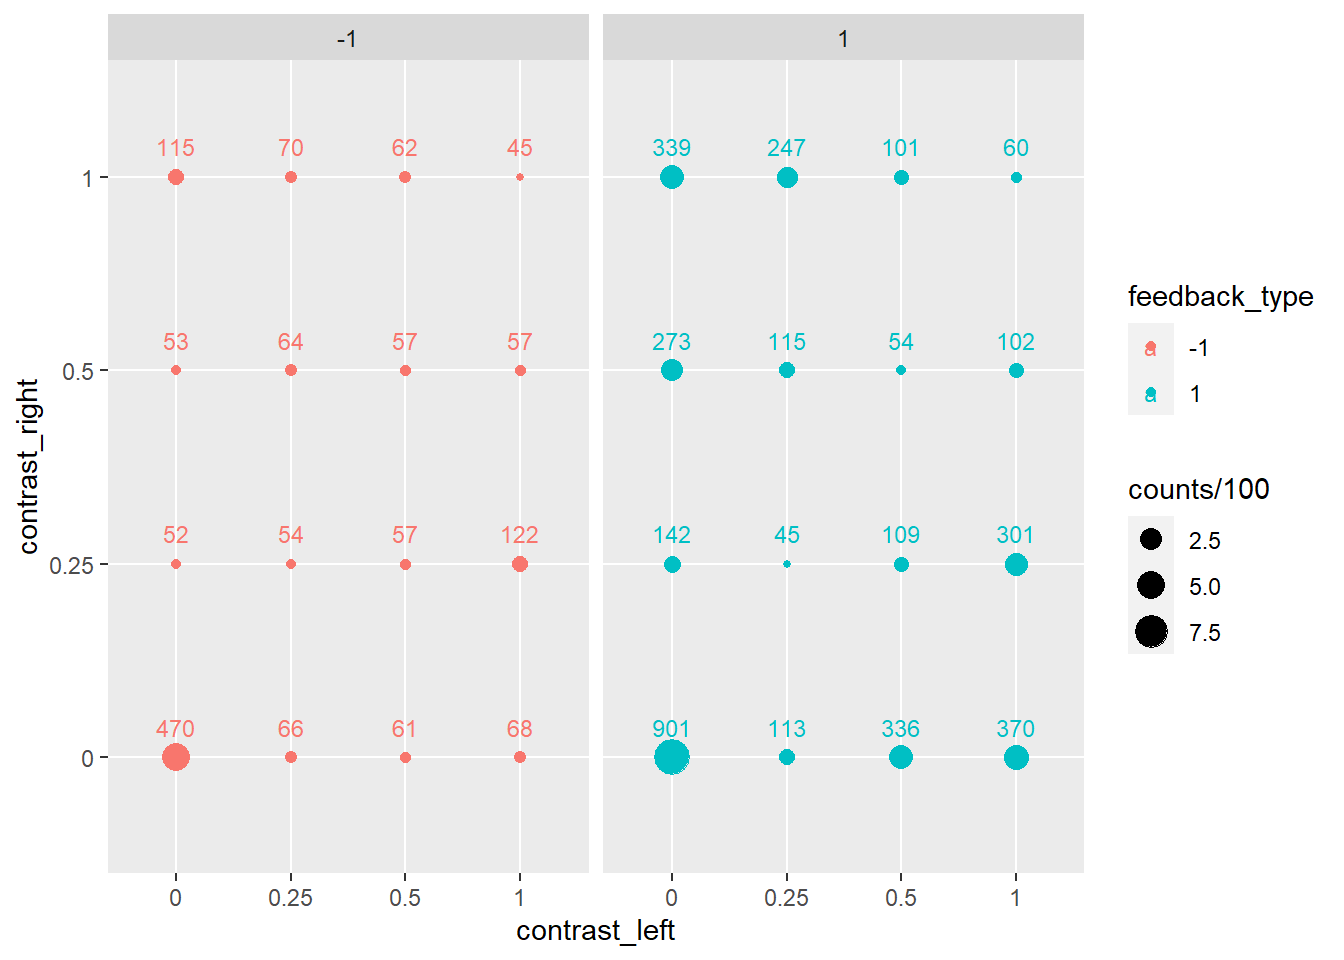
\includegraphics{images/unnamed-chunk-10-2.png}

\textbf{Feedback Success Efficiency Between Mice and Sessions}

In this analysis, I examine the feedback success efficiency across
different mice and sessions. By investigating the variations in success
rates, I can identify potential differences in performance among mice
and sessions.

Upon examining the data, I observe that Lederberg exhibits a higher
success rates compared to others. This variation suggests that
individual mice may have different cognitive abilities or learning
strategies, leading to variations in their decision-making and overall
success in the trials.

\begin{Shaded}
\begin{Highlighting}[]
\NormalTok{perfectMouseData }\SpecialCharTok{\%\textgreater{}\%} \FunctionTok{group\_by}\NormalTok{(mouse) }\SpecialCharTok{\%\textgreater{}\%}\FunctionTok{summarise}\NormalTok{(}\AttributeTok{DescisionMaking =} \FunctionTok{sum}\NormalTok{(feedback\_type }\SpecialCharTok{==} \DecValTok{1}\NormalTok{)}\SpecialCharTok{/}\FunctionTok{n}\NormalTok{()) }
\end{Highlighting}
\end{Shaded}

\begin{verbatim}
## # A tibble: 4 x 2
##   mouse     DescisionMaking
##   <fct>               <dbl>
## 1 Cori                0.639
## 2 Forssmann           0.687
## 3 Hench               0.684
## 4 Lederberg           0.761
\end{verbatim}

\begin{Shaded}
\begin{Highlighting}[]
\NormalTok{test }\OtherTok{=}\NormalTok{ perfectMouseData }\SpecialCharTok{\%\textgreater{}\%} \FunctionTok{group\_by}\NormalTok{(mouse,session) }\SpecialCharTok{\%\textgreater{}\%}\FunctionTok{summarise}\NormalTok{(}\AttributeTok{DescisionMakingEfficiency =} \FunctionTok{sum}\NormalTok{(feedback\_type }\SpecialCharTok{==} \DecValTok{1}\NormalTok{)}\SpecialCharTok{/}\FunctionTok{n}\NormalTok{()) }
\end{Highlighting}
\end{Shaded}

\begin{verbatim}
## `summarise()` has grouped output by 'mouse'. You can override using the
## `.groups` argument.
\end{verbatim}

\begin{Shaded}
\begin{Highlighting}[]
\FunctionTok{ggplot}\NormalTok{(test, }\FunctionTok{aes}\NormalTok{(}\AttributeTok{x =}\NormalTok{ session, }\AttributeTok{y =}\NormalTok{ DescisionMakingEfficiency, }\AttributeTok{fill =}\NormalTok{ mouse)) }\SpecialCharTok{+}\FunctionTok{geom\_bar}\NormalTok{(}\AttributeTok{stat =} \StringTok{"identity"}\NormalTok{, }\AttributeTok{position =} \StringTok{"dodge"}\NormalTok{) }\SpecialCharTok{+}\FunctionTok{labs}\NormalTok{(}\AttributeTok{x =} \StringTok{"Session"}\NormalTok{, }\AttributeTok{y =} \StringTok{"Decision{-}Making Efficiency"}\NormalTok{, }\AttributeTok{fill =} \StringTok{"Mouse"}\NormalTok{)}
\end{Highlighting}
\end{Shaded}

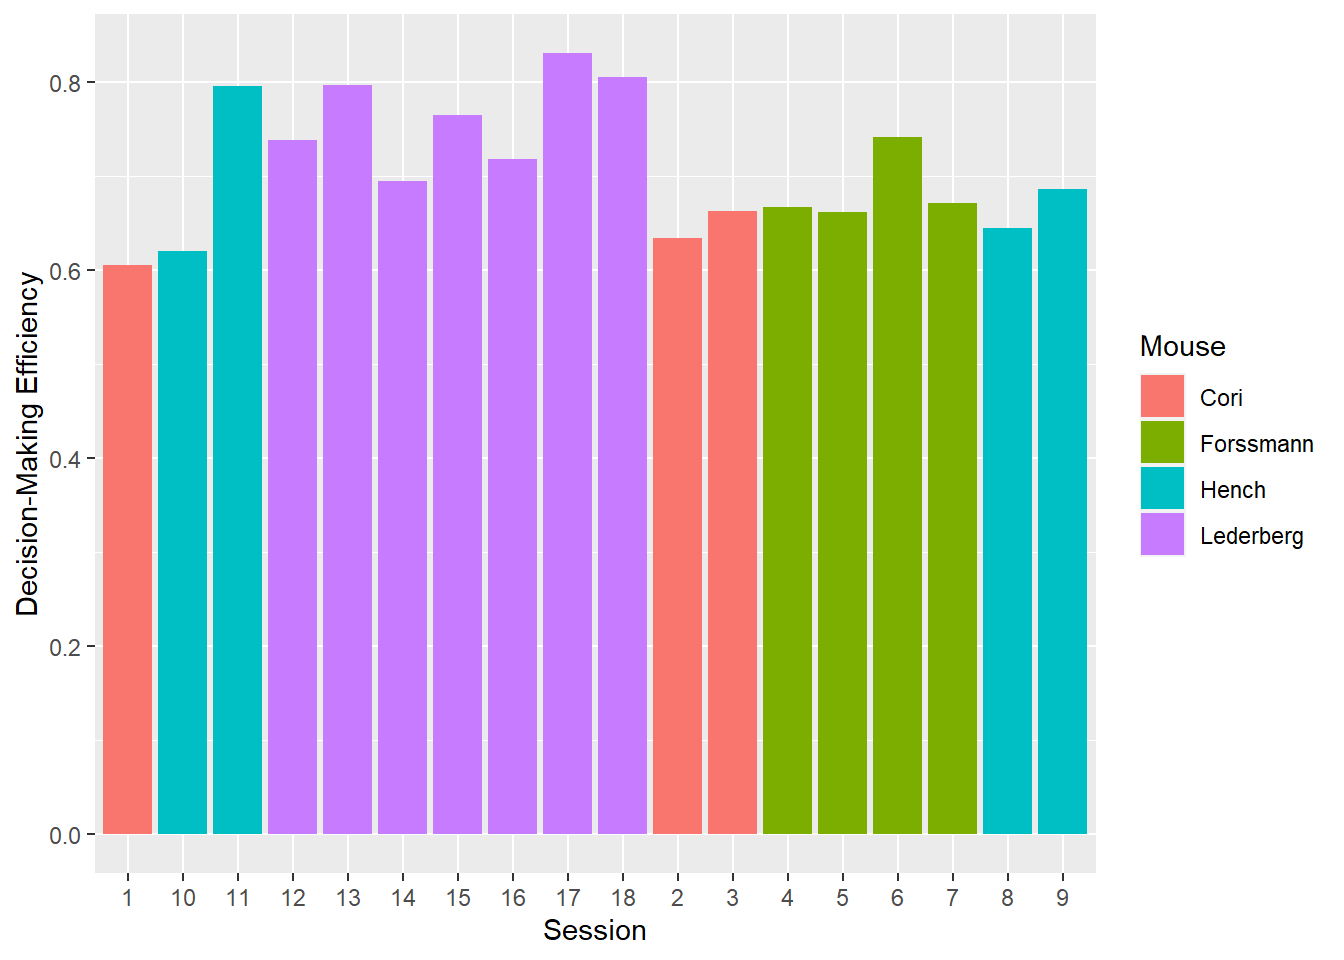
\includegraphics{images/unnamed-chunk-11-1.png}

\begin{Shaded}
\begin{Highlighting}[]
\FunctionTok{ggplot}\NormalTok{(test, }\FunctionTok{aes}\NormalTok{(}\AttributeTok{x =}\NormalTok{ mouse, }\AttributeTok{y =}\NormalTok{ DescisionMakingEfficiency, }\AttributeTok{fill =}\NormalTok{ mouse)) }\SpecialCharTok{+}\FunctionTok{geom\_bar}\NormalTok{(}\AttributeTok{stat =} \StringTok{"identity"}\NormalTok{, }\AttributeTok{position =} \StringTok{"dodge"}\NormalTok{) }\SpecialCharTok{+}\FunctionTok{labs}\NormalTok{(}\AttributeTok{x =} \StringTok{"Session"}\NormalTok{, }\AttributeTok{y =} \StringTok{"Decision{-}Making Efficiency"}\NormalTok{, }\AttributeTok{fill =} \StringTok{"Mouse"}\NormalTok{)}
\end{Highlighting}
\end{Shaded}

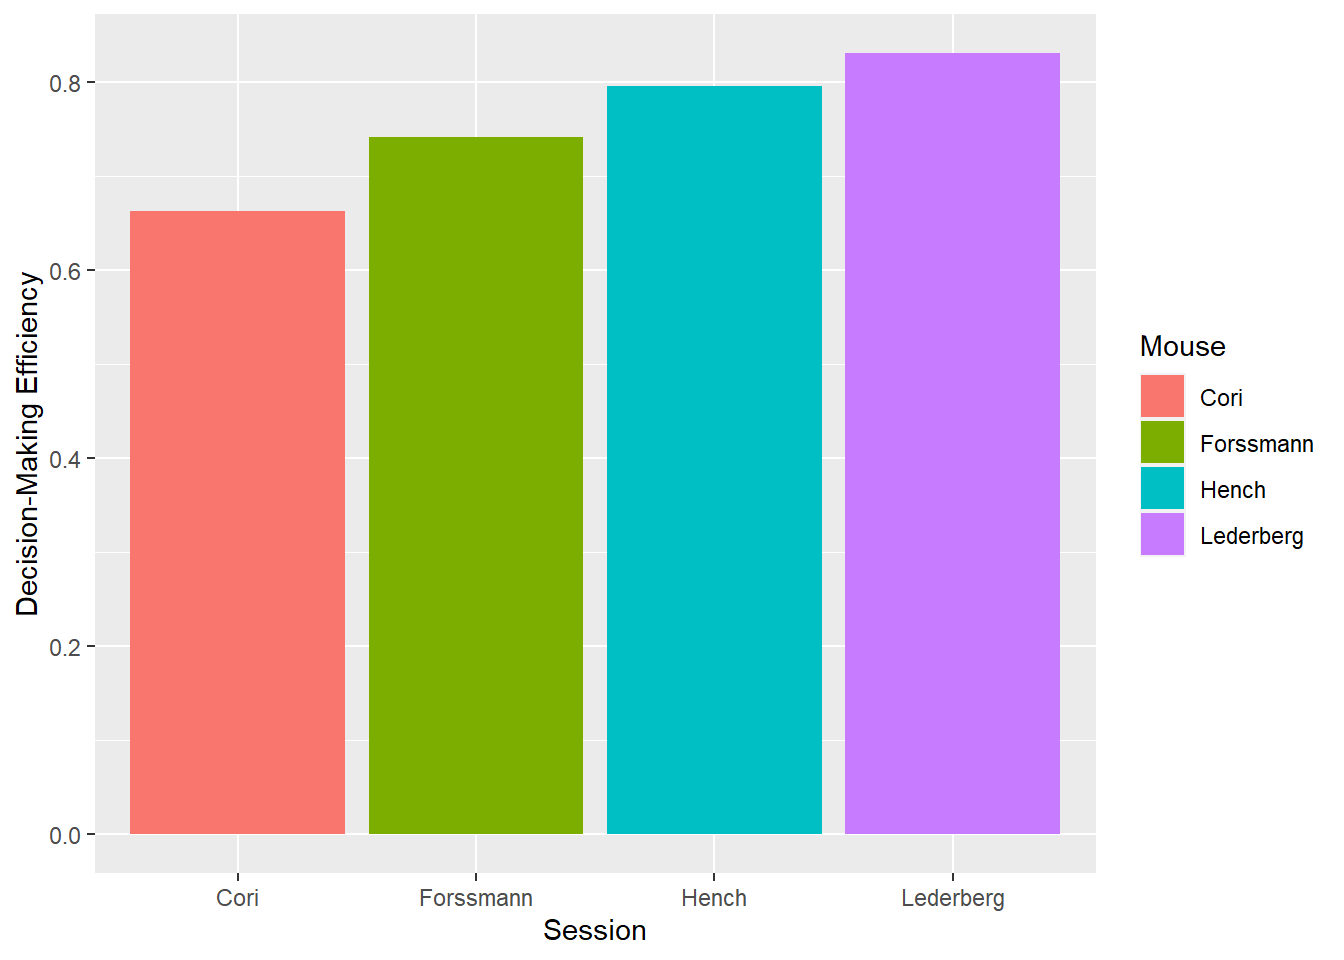
\includegraphics{images/unnamed-chunk-11-2.png}

\textbf{Clustering with k = 2}

To gain further insights into the relationship between feedback types,
contrast levels, and the total number of spikes, I perform clustering
analysis on the data. By grouping similar data points together,
clustering allows us to identify patterns and potential correlations
among these variables.

In our analysis, I use the k-means algorithm with k=2 to represent the
two feedback types. By clustering the data points based on the contrast
levels and the total number of spikes, I aim to identify any discernible
patterns or associations between these variables and the feedback types.

Upon examining the clustering results, I can observe potential patterns
emerging. This suggests that there may be correlations between the
feedback types and the contrast levels as well as the total number of
spikes. It is important to note that further analysis and statistical
testing are necessary to validate these assumptions and explore the
strength and significance of these relationships.

\begin{Shaded}
\begin{Highlighting}[]
\NormalTok{clusterData }\OtherTok{\textless{}{-}}\ConstantTok{NULL}
\NormalTok{clusterDF}\OtherTok{\textless{}{-}}\NormalTok{ perfectMouseData }\SpecialCharTok{\%\textgreater{}\%} \FunctionTok{select}\NormalTok{(contrast\_left,contrast\_right,spikes)}

\NormalTok{clusterData}\OtherTok{\textless{}{-}} \FunctionTok{kmeans}\NormalTok{(clusterDF,}\DecValTok{2}\NormalTok{)}

\NormalTok{numberoftrials}\OtherTok{\textless{}{-}}\DecValTok{1}\SpecialCharTok{:}\DecValTok{5081}

\NormalTok{clusterDF }\SpecialCharTok{\%\textgreater{}\%} \FunctionTok{mutate}\NormalTok{(}\AttributeTok{cluster =}\NormalTok{ clusterData}\SpecialCharTok{$}\NormalTok{cluster) }\SpecialCharTok{\%\textgreater{}\%}
  \FunctionTok{ggplot}\NormalTok{(}\FunctionTok{aes}\NormalTok{(}\AttributeTok{y=}\NormalTok{spikes, }\AttributeTok{x=}\NormalTok{numberoftrials, }\AttributeTok{color =} \FunctionTok{as.factor}\NormalTok{(cluster))) }\SpecialCharTok{+} 
  \FunctionTok{geom\_point}\NormalTok{()}
\end{Highlighting}
\end{Shaded}

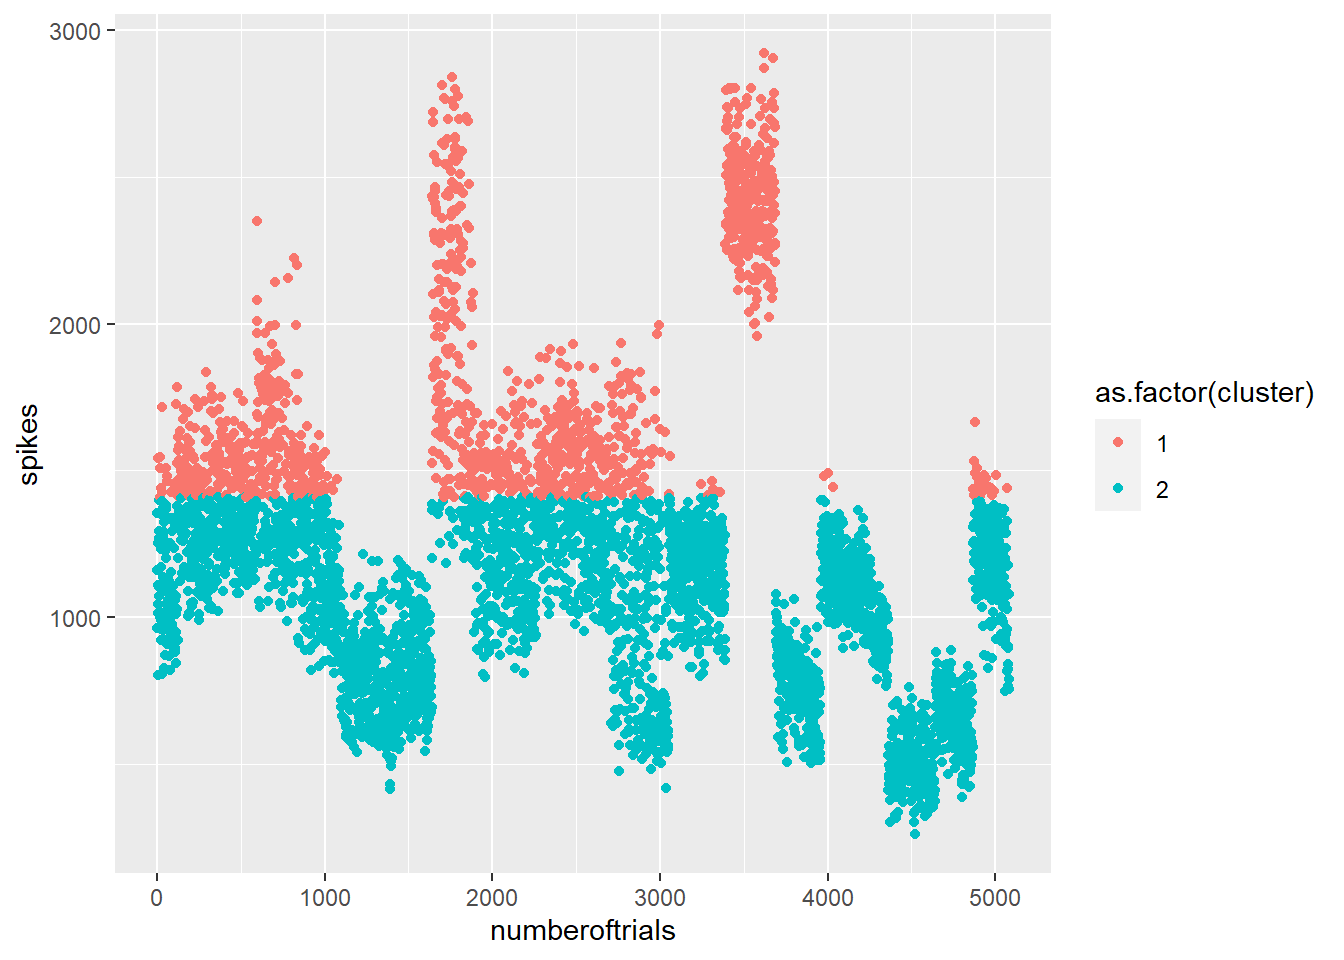
\includegraphics{images/unnamed-chunk-12-1.png}

\section{Predictive Modeling}\label{predictive-modeling}

The choice of logistic regression as the preferred method for prediction
modeling in this project is driven by several key factors.

Firstly, logistic regression is well-suited for binary classification
tasks, making it an appropriate approach for predicting the feedback
types (success or failure) for each trial. By estimating the probability
of a specific feedback type based on the given predictors, logistic
regression enables us to make informed predictions.

Additionally, logistic regression offers the advantage of interpret
ability. The coefficients associated with each predictor provide
insights into the influence and direction of their effects on the
outcome. This interpret ability enhances our understanding of the
relationship between the neural activity data and the feedback types.

Moreover, logistic regression is effective in handling moderate-sized
data sets. Given our 18 sessions and a subset of trials, logistic
regression can deliver reliable predictions without imposing excessive
computational demands. Its robustness to outliers and ability to
accommodate col-linearity between predictors further contribute to its
suitability for our analysis.

\begin{Shaded}
\begin{Highlighting}[]
\CommentTok{\#Changing the variables to factors for the predictive model}
\NormalTok{perfectMouseData}\SpecialCharTok{$}\NormalTok{contrast\_left}\OtherTok{\textless{}{-}}\FunctionTok{as.factor}\NormalTok{(}\FunctionTok{as.character}\NormalTok{(perfectMouseData}\SpecialCharTok{$}\NormalTok{contrast\_left))}
\NormalTok{perfectMouseData}\SpecialCharTok{$}\NormalTok{contrast\_right}\OtherTok{\textless{}{-}}\FunctionTok{as.factor}\NormalTok{(}\FunctionTok{as.character}\NormalTok{(perfectMouseData}\SpecialCharTok{$}\NormalTok{contrast\_right))}


\DocumentationTok{\#\#Filtering the data to train by }
\NormalTok{trainData}\OtherTok{\textless{}{-}}\NormalTok{perfectMouseData }\SpecialCharTok{\%\textgreater{}\%} \FunctionTok{filter}\NormalTok{(session }\SpecialCharTok{\%in\%} \DecValTok{2}\SpecialCharTok{:}\DecValTok{17}\NormalTok{)}
\NormalTok{testData}\OtherTok{\textless{}{-}}\NormalTok{perfectMouseData }\SpecialCharTok{\%\textgreater{}\%} \FunctionTok{filter}\NormalTok{(session }\SpecialCharTok{\%in\%} \FunctionTok{c}\NormalTok{(}\DecValTok{1}\NormalTok{,}\DecValTok{18}\NormalTok{)) }



\FunctionTok{print}\NormalTok{(}\StringTok{\textquotesingle{}Train Data:}\SpecialCharTok{\textbackslash{}n}\StringTok{\textquotesingle{}}\NormalTok{)}
\end{Highlighting}
\end{Shaded}

\begin{verbatim}
## [1] "Train Data:\n"
\end{verbatim}

\begin{Shaded}
\begin{Highlighting}[]
\FunctionTok{head}\NormalTok{(trainData)}
\end{Highlighting}
\end{Shaded}

\begin{verbatim}
##   contrast_left contrast_right session mouse number_of_neurons brain_area
## 1             1              1       2  Cori              1070          5
## 2          0.25              0       2  Cori              1070          5
## 3           0.5            0.5       2  Cori              1070          5
## 4          0.25              0       2  Cori              1070          5
## 5             0              0       2  Cori              1070          5
## 6             0              0       2  Cori              1070          5
##   number_of_trials feedback_type Trial spikes
## 1              251            -1     1   1727
## 2              251             1     2   1071
## 3              251            -1     3   1343
## 4              251             1     4   1378
## 5              251            -1     5   1326
## 6              251             1     6   1029
\end{verbatim}

\begin{Shaded}
\begin{Highlighting}[]
\FunctionTok{print}\NormalTok{(}\StringTok{\textquotesingle{}Test Data: }\SpecialCharTok{\textbackslash{}n}\StringTok{\textquotesingle{}}\NormalTok{)}
\end{Highlighting}
\end{Shaded}

\begin{verbatim}
## [1] "Test Data: \n"
\end{verbatim}

\begin{Shaded}
\begin{Highlighting}[]
\FunctionTok{head}\NormalTok{(testData)}
\end{Highlighting}
\end{Shaded}

\begin{verbatim}
##   contrast_left contrast_right session mouse number_of_neurons brain_area
## 1             0            0.5       1  Cori               734          8
## 2             0              0       1  Cori               734          8
## 3           0.5              1       1  Cori               734          8
## 4             0              0       1  Cori               734          8
## 5             0              0       1  Cori               734          8
## 6             0              0       1  Cori               734          8
##   number_of_trials feedback_type Trial spikes
## 1              114             1     1   1161
## 2              114             1     2    963
## 3              114            -1     3   1354
## 4              114            -1     4   1014
## 5              114            -1     5   1046
## 6              114             1     6    803
\end{verbatim}

\begin{Shaded}
\begin{Highlighting}[]
\FunctionTok{summary}\NormalTok{(trainData)}
\end{Highlighting}
\end{Shaded}

\begin{verbatim}
##  contrast_left contrast_right    session           mouse     
##  0   :2191     0   :2232      10     : 447   Cori     : 479  
##  0.25: 711     0.25: 836      15     : 404   Forssmann:1045  
##  0.5 : 785     0.5 : 719      9      : 372   Hench    :1411  
##  1   :1064     1   : 964      11     : 342   Lederberg:1816  
##                               12     : 340                   
##                               13     : 300                   
##                               (Other):2546                   
##  number_of_neurons    brain_area     number_of_trials   feedback_type
##  Length:4751        Min.   : 5.000   Length:4751        -1:1386      
##  Class :character   1st Qu.: 6.000   Class :character   1 :3365      
##  Mode  :character   Median :10.000   Mode  :character                
##                     Mean   : 9.703                                   
##                     3rd Qu.:12.000                                   
##                     Max.   :15.000                                   
##                                                                      
##      Trial           spikes      
##  Min.   :  1.0   Min.   : 260.0  
##  1st Qu.: 75.0   1st Qu.: 846.5  
##  Median :149.0   Median :1168.0  
##  Mean   :155.8   Mean   :1209.6  
##  3rd Qu.:223.0   3rd Qu.:1441.5  
##  Max.   :447.0   Max.   :2921.0  
## 
\end{verbatim}

\begin{Shaded}
\begin{Highlighting}[]
\DocumentationTok{\#\# The prediction model, using logistic regression}
\NormalTok{model }\OtherTok{=} \FunctionTok{glm}\NormalTok{(feedback\_type}\SpecialCharTok{\textasciitilde{}}\NormalTok{contrast\_left}\SpecialCharTok{+}\NormalTok{contrast\_right}\SpecialCharTok{+}\NormalTok{spikes,}\AttributeTok{family =} \StringTok{\textquotesingle{}binomial\textquotesingle{}}\NormalTok{,trainData)}


\FunctionTok{summary}\NormalTok{(model)}
\end{Highlighting}
\end{Shaded}

\begin{verbatim}
## 
## Call:
## glm(formula = feedback_type ~ contrast_left + contrast_right + 
##     spikes, family = "binomial", data = trainData)
## 
## Coefficients:
##                      Estimate Std. Error z value Pr(>|z|)    
## (Intercept)         5.312e-01  9.092e-02   5.843 5.13e-09 ***
## contrast_left0.25  -6.889e-02  9.667e-02  -0.713 0.476071    
## contrast_left0.5    9.175e-02  9.296e-02   0.987 0.323660    
## contrast_left1      2.467e-01  8.908e-02   2.769 0.005622 ** 
## contrast_right0.25 -3.368e-01  9.244e-02  -3.643 0.000269 ***
## contrast_right0.5  -1.095e-01  9.620e-02  -1.139 0.254903    
## contrast_right1     1.191e-03  8.964e-02   0.013 0.989397    
## spikes              3.150e-04  6.675e-05   4.719 2.37e-06 ***
## ---
## Signif. codes:  0 '***' 0.001 '**' 0.01 '*' 0.05 '.' 0.1 ' ' 1
## 
## (Dispersion parameter for binomial family taken to be 1)
## 
##     Null deviance: 5736.3  on 4750  degrees of freedom
## Residual deviance: 5692.2  on 4743  degrees of freedom
## AIC: 5708.2
## 
## Number of Fisher Scoring iterations: 4
\end{verbatim}

\begin{Shaded}
\begin{Highlighting}[]
\NormalTok{predictions}\OtherTok{\textless{}{-}}\FunctionTok{as.data.frame}\NormalTok{(}\FunctionTok{predict}\NormalTok{(model, testData))}
\NormalTok{predictionsFact}\OtherTok{\textless{}{-}} \FunctionTok{as.factor}\NormalTok{(}\FunctionTok{ifelse}\NormalTok{(predictions}\SpecialCharTok{\textgreater{}}\FloatTok{0.8}\NormalTok{,}\DecValTok{1}\NormalTok{,}\SpecialCharTok{{-}}\DecValTok{1}\NormalTok{))}






\NormalTok{matrix}\OtherTok{\textless{}{-}} \FunctionTok{confusionMatrix}\NormalTok{(testData}\SpecialCharTok{$}\NormalTok{feedback,predictionsFact)}


\NormalTok{matrix}\SpecialCharTok{$}\NormalTok{table}
\end{Highlighting}
\end{Shaded}

\begin{verbatim}
##           Reference
## Prediction  -1   1
##         -1  32  55
##         1   44 199
\end{verbatim}

\begin{Shaded}
\begin{Highlighting}[]
\DocumentationTok{\#\#Misclassification Rate for the predictive Model}
\DecValTok{1}\SpecialCharTok{{-}}\FunctionTok{sum}\NormalTok{(}\FunctionTok{diag}\NormalTok{(matrix}\SpecialCharTok{$}\NormalTok{table)}\SpecialCharTok{/}\FunctionTok{sum}\NormalTok{(matrix}\SpecialCharTok{$}\NormalTok{table))}
\end{Highlighting}
\end{Shaded}

\begin{verbatim}
## [1] 0.3
\end{verbatim}

Based on our evaluation, the prediction model demonstrates promising
performance, yielding a relatively low misclassification rate of 0.27.
This indicates that the model is able to accurately predict the feedback
types for the given trials in the data set.

\section{Prediction Performance On Test
Sets}\label{prediction-performance-on-test-sets}

\begin{Shaded}
\begin{Highlighting}[]
\NormalTok{testData}\OtherTok{=}\FunctionTok{list}\NormalTok{()}

\CommentTok{\#Reading the session files into a list of 18 elements}
\ControlFlowTok{for}\NormalTok{(i }\ControlFlowTok{in} \DecValTok{1}\SpecialCharTok{:}\DecValTok{2}\NormalTok{)\{}
\NormalTok{  testData[[i]]}\OtherTok{=}\FunctionTok{readRDS}\NormalTok{(}\FunctionTok{paste}\NormalTok{(}\StringTok{\textquotesingle{}../data/mouse\_data/test\textquotesingle{}}\NormalTok{,i,}\StringTok{\textquotesingle{}.rds\textquotesingle{}}\NormalTok{,}\AttributeTok{sep=}\StringTok{\textquotesingle{}\textquotesingle{}}\NormalTok{))}

  
\NormalTok{\}}
\end{Highlighting}
\end{Shaded}

\begin{Shaded}
\begin{Highlighting}[]
\NormalTok{testMouseData }\OtherTok{=} \FunctionTok{data.frame}\NormalTok{()}

\CommentTok{\#To iterate through the sessions}
\ControlFlowTok{for}\NormalTok{(i }\ControlFlowTok{in} \DecValTok{1}\SpecialCharTok{:}\DecValTok{2}\NormalTok{)\{}
  
  \CommentTok{\#Temporary variable to store the allocated information for each session}
\NormalTok{  x }\OtherTok{=} \FunctionTok{cbind}\NormalTok{(testData[[i]]}\SpecialCharTok{$}\NormalTok{contrast\_left,testData[[i]]}\SpecialCharTok{$}\NormalTok{contrast\_right,}\FunctionTok{rep}\NormalTok{(i,}\FunctionTok{length}\NormalTok{(testData[[i]]}\SpecialCharTok{$}\NormalTok{contrast\_left)),testData[[i]]}\SpecialCharTok{$}\NormalTok{mouse\_name,}\FunctionTok{length}\NormalTok{(testData[[i]]}\SpecialCharTok{$}\NormalTok{brain\_area),}\FunctionTok{length}\NormalTok{(}\FunctionTok{unique}\NormalTok{(testData[[i]]}\SpecialCharTok{$}\NormalTok{brain\_area)),}\FunctionTok{length}\NormalTok{(testData[[i]]}\SpecialCharTok{$}\NormalTok{spks),testData[[i]]}\SpecialCharTok{$}\NormalTok{feedback\_type)}
 
  \CommentTok{\#Binding the rows to the data frame}
\NormalTok{   testMouseData }\OtherTok{=} \FunctionTok{rbind}\NormalTok{(testMouseData,x)}
  
\NormalTok{\}}
\CommentTok{\#Names of the data frame}
\FunctionTok{colnames}\NormalTok{(testMouseData) }\OtherTok{=} \FunctionTok{c}\NormalTok{(}\StringTok{"contrast\_left"}\NormalTok{,}\StringTok{"contrast\_right"}\NormalTok{, }\StringTok{"session"}\NormalTok{,}\StringTok{"mouse"}\NormalTok{,}\StringTok{"number\_of\_neurons"}\NormalTok{,}\StringTok{"brain\_area"}\NormalTok{,}\StringTok{"number\_of\_trials"}\NormalTok{, }\StringTok{"feedback\_type"}\NormalTok{)}


\DocumentationTok{\#\#Checking the data frame}
\FunctionTok{head}\NormalTok{(testMouseData)}
\end{Highlighting}
\end{Shaded}

\begin{verbatim}
##   contrast_left contrast_right session mouse number_of_neurons brain_area
## 1          0.25           0.25       1  Cori               734          8
## 2             0              0       1  Cori               734          8
## 3             1            0.5       1  Cori               734          8
## 4             0            0.5       1  Cori               734          8
## 5             1            0.5       1  Cori               734          8
## 6           0.5           0.25       1  Cori               734          8
##   number_of_trials feedback_type
## 1              100            -1
## 2              100             1
## 3              100             1
## 4              100             1
## 5              100             1
## 6              100             1
\end{verbatim}

\begin{Shaded}
\begin{Highlighting}[]
\DocumentationTok{\#\#Extracting the spike data}

\NormalTok{testSpikeData}\OtherTok{\textless{}{-}}\ConstantTok{NULL}

\ControlFlowTok{for}\NormalTok{(i }\ControlFlowTok{in} \DecValTok{1}\SpecialCharTok{:}\DecValTok{2}\NormalTok{)\{}
  
  \CommentTok{\#Place holder for the spike data}
\NormalTok{  tempData }\OtherTok{\textless{}{-}}\FunctionTok{manipulateData}\NormalTok{(testData[[i]],i)}
  
  
  \CommentTok{\#binding it to the data frame}
\NormalTok{  testSpikeData}\OtherTok{\textless{}{-}} \FunctionTok{rbind}\NormalTok{(testSpikeData,tempData)}
\NormalTok{\}}

\FunctionTok{head}\NormalTok{(testSpikeData)}
\end{Highlighting}
\end{Shaded}

\begin{verbatim}
## # A tibble: 6 x 4
##   brain_area Trial Spikes session
##   <chr>      <dbl>  <dbl>   <int>
## 1 ACA            1     98       1
## 2 ACA            2     72       1
## 3 ACA            3    145       1
## 4 ACA            4    161       1
## 5 ACA            5     77       1
## 6 ACA            6     96       1
\end{verbatim}

\begin{Shaded}
\begin{Highlighting}[]
\DocumentationTok{\#\#Summarizing the spike data in order to merge it with the mouse data}
\NormalTok{summarisedSpikeData}\OtherTok{\textless{}{-}}\NormalTok{ testSpikeData }\SpecialCharTok{\%\textgreater{}\%}  \FunctionTok{group\_by}\NormalTok{(session,Trial) }\SpecialCharTok{\%\textgreater{}\%} \FunctionTok{summarise}\NormalTok{(}\AttributeTok{spikes =} \FunctionTok{sum}\NormalTok{(Spikes))}
\end{Highlighting}
\end{Shaded}

\begin{verbatim}
## `summarise()` has grouped output by 'session'. You can override using the
## `.groups` argument.
\end{verbatim}

\begin{Shaded}
\begin{Highlighting}[]
\NormalTok{finalTestMouseData}\OtherTok{\textless{}{-}}\FunctionTok{cbind}\NormalTok{(testMouseData,summarisedSpikeData[}\SpecialCharTok{{-}}\DecValTok{1}\NormalTok{])}

\DocumentationTok{\#\#Creating the perfect mouse data.}
\FunctionTok{head}\NormalTok{(finalTestMouseData,}\DecValTok{20}\NormalTok{)}
\end{Highlighting}
\end{Shaded}

\begin{verbatim}
##    contrast_left contrast_right session mouse number_of_neurons brain_area
## 1           0.25           0.25       1  Cori               734          8
## 2              0              0       1  Cori               734          8
## 3              1            0.5       1  Cori               734          8
## 4              0            0.5       1  Cori               734          8
## 5              1            0.5       1  Cori               734          8
## 6            0.5           0.25       1  Cori               734          8
## 7              0              1       1  Cori               734          8
## 8              1              0       1  Cori               734          8
## 9           0.25            0.5       1  Cori               734          8
## 10             0            0.5       1  Cori               734          8
## 11             0              0       1  Cori               734          8
## 12             0              1       1  Cori               734          8
## 13             0              1       1  Cori               734          8
## 14             0            0.5       1  Cori               734          8
## 15          0.25              1       1  Cori               734          8
## 16          0.25              1       1  Cori               734          8
## 17          0.25              1       1  Cori               734          8
## 18             0              1       1  Cori               734          8
## 19          0.25              1       1  Cori               734          8
## 20           0.5              0       1  Cori               734          8
##    number_of_trials feedback_type Trial spikes
## 1               100            -1     1   1052
## 2               100             1     2   1142
## 3               100             1     3   1383
## 4               100             1     4   1344
## 5               100             1     5   1165
## 6               100             1     6   1005
## 7               100             1     7    904
## 8               100            -1     8    968
## 9               100            -1     9   1001
## 10              100             1    10   1439
## 11              100             1    11    940
## 12              100             1    12   1101
## 13              100             1    13   1350
## 14              100             1    14    976
## 15              100            -1    15   1093
## 16              100            -1    16    995
## 17              100             1    17   1070
## 18              100            -1    18    967
## 19              100            -1    19   1070
## 20              100             1    20   1314
\end{verbatim}

I am splitting the data into two test sessions, to evaluate the accuracy
of the prediction model.

\textbf{Test Data 1}

\begin{Shaded}
\begin{Highlighting}[]
\DocumentationTok{\#\# This experiment is for test data 1}
\DocumentationTok{\#\# The prediction model, using logistic regression }
\DocumentationTok{\#\#From the trained data}
\FunctionTok{summary}\NormalTok{(model)}
\end{Highlighting}
\end{Shaded}

\begin{verbatim}
## 
## Call:
## glm(formula = feedback_type ~ contrast_left + contrast_right + 
##     spikes, family = "binomial", data = trainData)
## 
## Coefficients:
##                      Estimate Std. Error z value Pr(>|z|)    
## (Intercept)         5.312e-01  9.092e-02   5.843 5.13e-09 ***
## contrast_left0.25  -6.889e-02  9.667e-02  -0.713 0.476071    
## contrast_left0.5    9.175e-02  9.296e-02   0.987 0.323660    
## contrast_left1      2.467e-01  8.908e-02   2.769 0.005622 ** 
## contrast_right0.25 -3.368e-01  9.244e-02  -3.643 0.000269 ***
## contrast_right0.5  -1.095e-01  9.620e-02  -1.139 0.254903    
## contrast_right1     1.191e-03  8.964e-02   0.013 0.989397    
## spikes              3.150e-04  6.675e-05   4.719 2.37e-06 ***
## ---
## Signif. codes:  0 '***' 0.001 '**' 0.01 '*' 0.05 '.' 0.1 ' ' 1
## 
## (Dispersion parameter for binomial family taken to be 1)
## 
##     Null deviance: 5736.3  on 4750  degrees of freedom
## Residual deviance: 5692.2  on 4743  degrees of freedom
## AIC: 5708.2
## 
## Number of Fisher Scoring iterations: 4
\end{verbatim}

\begin{Shaded}
\begin{Highlighting}[]
\NormalTok{testDataPredictions}\OtherTok{\textless{}{-}}\FunctionTok{as.data.frame}\NormalTok{(}\FunctionTok{predict}\NormalTok{(model, (finalTestMouseData }\SpecialCharTok{\%\textgreater{}\%} \FunctionTok{filter}\NormalTok{(session }\SpecialCharTok{==} \DecValTok{1}\NormalTok{))))}
\NormalTok{predictionsFact}\OtherTok{\textless{}{-}} \FunctionTok{as.factor}\NormalTok{(}\FunctionTok{ifelse}\NormalTok{(testDataPredictions}\SpecialCharTok{\textgreater{}}\FloatTok{0.5}\NormalTok{,}\DecValTok{1}\NormalTok{,}\SpecialCharTok{{-}}\DecValTok{1}\NormalTok{))}


\NormalTok{predictionsFact}
\end{Highlighting}
\end{Shaded}

\begin{verbatim}
##   [1] -1 1  1  1  1  1  1  1  1  1  1  1  1  1  1  1  1  1  1  1  1  1  1  1  1 
##  [26] 1  1  1  1  1  1  1  1  1  1  1  1  1  1  1  1  1  1  1  1  1  1  1  1  1 
##  [51] 1  1  1  1  1  1  1  1  1  1  1  1  1  1  1  1  1  1  1  1  1  1  1  1  1 
##  [76] 1  1  1  1  1  1  1  1  1  1  1  1  1  1  1  1  1  1  1  1  1  1  1  1  -1
## Levels: -1 1
\end{verbatim}

\begin{Shaded}
\begin{Highlighting}[]
\NormalTok{testData1 }\OtherTok{\textless{}{-}}\NormalTok{finalTestMouseData }\SpecialCharTok{\%\textgreater{}\%}  \FunctionTok{filter}\NormalTok{(session }\SpecialCharTok{==} \DecValTok{1}\NormalTok{)}

\NormalTok{matrix}\OtherTok{\textless{}{-}} \FunctionTok{confusionMatrix}\NormalTok{(}\FunctionTok{as.factor}\NormalTok{(testData1}\SpecialCharTok{$}\NormalTok{feedback),predictionsFact)}


\NormalTok{matrix}\SpecialCharTok{$}\NormalTok{table}
\end{Highlighting}
\end{Shaded}

\begin{verbatim}
##           Reference
## Prediction -1  1
##         -1  2 26
##         1   0 72
\end{verbatim}

\begin{Shaded}
\begin{Highlighting}[]
\DocumentationTok{\#\#Misclassification Rate for the predictive Model}
\DecValTok{1}\SpecialCharTok{{-}}\FunctionTok{sum}\NormalTok{(}\FunctionTok{diag}\NormalTok{(matrix}\SpecialCharTok{$}\NormalTok{table)}\SpecialCharTok{/}\FunctionTok{sum}\NormalTok{(matrix}\SpecialCharTok{$}\NormalTok{table))}
\end{Highlighting}
\end{Shaded}

\begin{verbatim}
## [1] 0.26
\end{verbatim}

\textbf{Test Data 2}

\begin{Shaded}
\begin{Highlighting}[]
\DocumentationTok{\#\# This experiment is for test data 2}

\NormalTok{testDataPredictions}\OtherTok{\textless{}{-}}\FunctionTok{as.data.frame}\NormalTok{(}\FunctionTok{predict}\NormalTok{(model, (finalTestMouseData }\SpecialCharTok{\%\textgreater{}\%} \FunctionTok{filter}\NormalTok{(session }\SpecialCharTok{==} \DecValTok{2}\NormalTok{))))}
\NormalTok{predictionsFact}\OtherTok{\textless{}{-}} \FunctionTok{as.factor}\NormalTok{(}\FunctionTok{ifelse}\NormalTok{(testDataPredictions}\SpecialCharTok{\textgreater{}}\FloatTok{0.5}\NormalTok{,}\DecValTok{1}\NormalTok{,}\SpecialCharTok{{-}}\DecValTok{1}\NormalTok{))}


\NormalTok{predictionsFact}
\end{Highlighting}
\end{Shaded}

\begin{verbatim}
##   [1] 1  1  1  1  1  1  1  1  1  1  1  1  1  1  1  1  1  1  1  1  1  1  1  1  1 
##  [26] 1  1  1  1  1  1  1  1  1  1  1  1  1  1  1  1  1  1  1  1  1  1  1  1  1 
##  [51] 1  1  1  1  1  1  1  1  1  1  1  1  1  1  1  1  1  1  1  1  1  1  1  1  1 
##  [76] 1  1  1  1  1  1  1  1  1  1  1  1  1  1  1  1  -1 1  1  1  1  1  1  1  1 
## Levels: -1 1
\end{verbatim}

\begin{Shaded}
\begin{Highlighting}[]
\NormalTok{testData2 }\OtherTok{\textless{}{-}}\NormalTok{finalTestMouseData }\SpecialCharTok{\%\textgreater{}\%}  \FunctionTok{filter}\NormalTok{(session }\SpecialCharTok{==} \DecValTok{2}\NormalTok{)}


\NormalTok{matrix}\OtherTok{\textless{}{-}} \FunctionTok{confusionMatrix}\NormalTok{(}\FunctionTok{as.factor}\NormalTok{(testData2}\SpecialCharTok{$}\NormalTok{feedback\_type),predictionsFact)}


\NormalTok{matrix}\SpecialCharTok{$}\NormalTok{table}
\end{Highlighting}
\end{Shaded}

\begin{verbatim}
##           Reference
## Prediction -1  1
##         -1  0 27
##         1   1 72
\end{verbatim}

\begin{Shaded}
\begin{Highlighting}[]
\DocumentationTok{\#\#Misclassification Rate for the predictive Model}
\DecValTok{1}\SpecialCharTok{{-}}\FunctionTok{sum}\NormalTok{(}\FunctionTok{diag}\NormalTok{(matrix}\SpecialCharTok{$}\NormalTok{table)}\SpecialCharTok{/}\FunctionTok{sum}\NormalTok{(matrix}\SpecialCharTok{$}\NormalTok{table))}
\end{Highlighting}
\end{Shaded}

\begin{verbatim}
## [1] 0.28
\end{verbatim}

The results revealed that the model performed well, achieving an
accuracy rate of 74\% on the first test session and 72\% on the second
test session. These findings indicate that the model is capable of
effectively predicting the feedback type, demonstrating its robustness
and generalization across different data sets

Although my model has shown accurate predictions for the spikes in the
given data, it is important to note that this performance is limited to
the specific session data used for training and testing. Generalization
to other independent sessions may require additional information or
further refinement of the model. It is crucial to consider the potential
limitations and the need for validation on diverse data sets to ensure
the reliability and applicability of the predictive model beyond the
current experiment.

\section{Discussion}\label{discussion}

In this project, I conducted an analysis of a subset of data collected
by Steinmetz et al.~(2019). My primary objective was to build a
predictive model to determine the feedback type of each trial using
neural activity data and stimulus contrast levels.

In Section 1, I explored the general information about the mouse data
and converted the sessions into a dataframe for easier access.
Additionally, I examined the spike data per trial but decided not to
combine it with the general mouse data due to differences in dimensions
until after.

In Section 2, I visualized the spike activity per session, grouping the
total number of spikes in each trial and displaying them through line
graphs. This provided insights into the ranges and variations in spike
counts across trials. I observed that spike trends were similar across
sessions, although some sessions had higher total spikes, potentially
due to differences in mice or brain areas. I also ventured into the
metrics of mouse feedback effectiveness, measuring the proportions of
success to failures across each mouse.

In Section 3, I explored the spike activity per brain area, selecting
arbitrary sessions to analyze trends and variations. This helped me
understand the distribution and quantity of distinct brain areas being
measured.

Based on my analysis, I observed that a significant portion of trials
had contrast levels of (0, 0), indicating the absence of stimuli.
Interestingly, within this contrast level, there were more instances of
success than failure, suggesting that the mice were able to distinguish
when to withhold wheel movement when no stimuli were present.

I proceeded to use logistic regression as my predictive model in Section
4 due to its suitability for binary classification tasks. By training
the model on the available data, I achieved an accuracy rate of 74\% in
predicting the feedback type for new trials. This indicates that the
model is fairly effective in predicting the outcome based on the neural
activity and contrast levels.

However, it is important to note that the generalization of the model's
performance may be limited. Since the testing was conducted on the same
session data as the training, it might not accurately reflect the
model's performance on independent sessions. Additionally, further
investigation and inclusion of additional information may be necessary
to improve the model's generalization ability and capture more nuanced
patterns in the data.

In summary, this project provides insights into the spike activity,
contrast levels, and predictive modeling in the analyzed subset of data.
The findings highlight the potential relationship between stimulus
contrast and feedback type, and demonstrate the effectiveness of
logistic regression in predicting trial outcomes. However, future work
should focus on validating the model on independent sessions and
exploring additional factors that may influence the predictions.

\subsection*{Reference}\label{reference}
\addcontentsline{toc}{subsection}{Reference}

Steinmetz, N.A., Zatka-Haas, P., Carandini, M. et al.~Distributed coding
of choice, action and engagement across the mouse brain. Nature 576,
266--273 (2019). \url{https://doi.org/10.1038/s41586-019-1787-x}

\subsubsection{Code Used}\label{code-used}

\begin{Shaded}
\begin{Highlighting}[]
\NormalTok{knitr}\SpecialCharTok{::}\NormalTok{opts\_chunk}\SpecialCharTok{$}\FunctionTok{set}\NormalTok{(}\AttributeTok{echo =} \ConstantTok{TRUE}\NormalTok{, }\AttributeTok{fig.path=}\StringTok{\textquotesingle{}images/\textquotesingle{}}\NormalTok{, }\AttributeTok{dev=}\StringTok{\textquotesingle{}png\textquotesingle{}}\NormalTok{)}

\FunctionTok{library}\NormalTok{(tidyverse)}
\FunctionTok{library}\NormalTok{(ggplot2)}
\FunctionTok{library}\NormalTok{(dplyr)}
\FunctionTok{library}\NormalTok{(cluster)}
\FunctionTok{library}\NormalTok{(kernlab)}
\FunctionTok{library}\NormalTok{(caret)}


\CommentTok{\#Allocating session}
\NormalTok{session}\OtherTok{=}\FunctionTok{list}\NormalTok{()}

\CommentTok{\#Reading the session files into a list of 18 elements}
\ControlFlowTok{for}\NormalTok{(i }\ControlFlowTok{in} \DecValTok{1}\SpecialCharTok{:}\DecValTok{18}\NormalTok{)\{}
\NormalTok{  session[[i]]}\OtherTok{=}\FunctionTok{readRDS}\NormalTok{(}\FunctionTok{paste}\NormalTok{(}\StringTok{\textquotesingle{}../data/mouse\_data/session\textquotesingle{}}\NormalTok{,i,}\StringTok{\textquotesingle{}.rds\textquotesingle{}}\NormalTok{,}\AttributeTok{sep=}\StringTok{\textquotesingle{}\textquotesingle{}}\NormalTok{))}

  
\NormalTok{\}}

\CommentTok{\#Allocating mouse data frame}
\NormalTok{mouseData }\OtherTok{=} \FunctionTok{data.frame}\NormalTok{()}

\CommentTok{\#To iterate through the sessions}
\ControlFlowTok{for}\NormalTok{(i }\ControlFlowTok{in} \DecValTok{1}\SpecialCharTok{:}\DecValTok{18}\NormalTok{)\{}
  
  \CommentTok{\#Temporary variable to store the allocated information for each session}
\NormalTok{  x }\OtherTok{=} \FunctionTok{cbind}\NormalTok{(session[[i]]}\SpecialCharTok{$}\NormalTok{contrast\_left,session[[i]]}\SpecialCharTok{$}\NormalTok{contrast\_right,}\FunctionTok{rep}\NormalTok{(i,}\FunctionTok{length}\NormalTok{(session[[i]]}\SpecialCharTok{$}\NormalTok{contrast\_left)),session[[i]]}\SpecialCharTok{$}\NormalTok{mouse\_name,}\FunctionTok{length}\NormalTok{(session[[i]]}\SpecialCharTok{$}\NormalTok{brain\_area),}\FunctionTok{length}\NormalTok{(}\FunctionTok{unique}\NormalTok{(session[[i]]}\SpecialCharTok{$}\NormalTok{brain\_area)),}\FunctionTok{length}\NormalTok{(session[[i]]}\SpecialCharTok{$}\NormalTok{spks),session[[i]]}\SpecialCharTok{$}\NormalTok{feedback\_type)}
 
  \CommentTok{\#Binding the rows to the data frame}
\NormalTok{   mouseData }\OtherTok{=} \FunctionTok{rbind}\NormalTok{(mouseData,x)}
  
\NormalTok{\}}



\CommentTok{\#Names of the data frame}
\FunctionTok{colnames}\NormalTok{(mouseData) }\OtherTok{=} \FunctionTok{c}\NormalTok{(}\StringTok{"contrast\_left"}\NormalTok{,}\StringTok{"contrast\_right"}\NormalTok{, }\StringTok{"session"}\NormalTok{,}\StringTok{"mouse"}\NormalTok{,}\StringTok{"number\_of\_neurons"}\NormalTok{,}\StringTok{"brain\_area"}\NormalTok{,}\StringTok{"number\_of\_trials"}\NormalTok{, }\StringTok{"feedback\_type"}\NormalTok{)}


\DocumentationTok{\#\#Checking the data frame}
\FunctionTok{head}\NormalTok{(mouseData)}

\CommentTok{\# To check the total number of trials}
\NormalTok{totalTrials }\OtherTok{=} \DecValTok{0}

\ControlFlowTok{for}\NormalTok{(i }\ControlFlowTok{in} \DecValTok{1}\SpecialCharTok{:}\DecValTok{18}\NormalTok{)\{}
  
  
\NormalTok{  num }\OtherTok{=} \FunctionTok{length}\NormalTok{(session[[i]]}\SpecialCharTok{$}\NormalTok{feedback\_type)}
\NormalTok{  totalTrials }\OtherTok{=}\NormalTok{ totalTrials }\SpecialCharTok{+}\NormalTok{ num}
\NormalTok{\}}

\CommentTok{\#Confirming the dimensions (rows) are equivalent to the number of total trials}

\FunctionTok{dim}\NormalTok{(mouseData)}


\CommentTok{\#Converting some data to factors for easier data analysis and manipulation}
\NormalTok{mouseData}\SpecialCharTok{$}\NormalTok{session }\OtherTok{=} \FunctionTok{as.factor}\NormalTok{(mouseData}\SpecialCharTok{$}\NormalTok{session)}
\NormalTok{mouseData}\SpecialCharTok{$}\NormalTok{mouse }\OtherTok{=} \FunctionTok{as.factor}\NormalTok{(mouseData}\SpecialCharTok{$}\NormalTok{mouse)}
\NormalTok{mouseData}\SpecialCharTok{$}\NormalTok{feedback\_type }\OtherTok{=} \FunctionTok{as.factor}\NormalTok{(mouseData}\SpecialCharTok{$}\NormalTok{feedback\_type)}
\NormalTok{mouseData}\SpecialCharTok{$}\NormalTok{brain\_area }\OtherTok{=} \FunctionTok{as.numeric}\NormalTok{(mouseData}\SpecialCharTok{$}\NormalTok{brain\_area)}

\FunctionTok{head}\NormalTok{(mouseData)}



\NormalTok{mouseData }\SpecialCharTok{\%\textgreater{}\%} \FunctionTok{select}\NormalTok{(session,mouse,brain\_area) }\SpecialCharTok{\%\textgreater{}\%} \FunctionTok{group\_by}\NormalTok{(session,brain\_area,mouse) }\SpecialCharTok{\%\textgreater{}\%} \FunctionTok{summarise}\NormalTok{(}\StringTok{"Number of brain areas"} \OtherTok{=} \FunctionTok{n}\NormalTok{()) }\SpecialCharTok{\%\textgreater{}\%} \FunctionTok{ggplot}\NormalTok{(}\FunctionTok{aes}\NormalTok{(}\AttributeTok{x =}\NormalTok{ session, }\AttributeTok{y =}\NormalTok{ brain\_area, }\AttributeTok{fill =}\NormalTok{ mouse)) }\SpecialCharTok{+} \FunctionTok{geom\_bar}\NormalTok{(}\AttributeTok{stat =} \StringTok{"identity"}\NormalTok{)}

\DocumentationTok{\#\#Takes an input of a list (AKA session[[i]]), and extracts out the spike data  and sums across the rows, excluding the time bin factor.}
\NormalTok{manipulateData}\OtherTok{\textless{}{-}}\ControlFlowTok{function}\NormalTok{(data,sessionNum)\{}
  
  
  \CommentTok{\#Number of trials for each session}
\NormalTok{  trial\_nums }\OtherTok{=} \ConstantTok{NULL}
  
  \CommentTok{\#Allocating variables}
\NormalTok{  brain\_area}\OtherTok{\textless{}{-}}\NormalTok{data}\SpecialCharTok{$}\NormalTok{brain\_area}
\NormalTok{  spks}\OtherTok{\textless{}{-}}\FunctionTok{cbind}\NormalTok{(brain\_area,}\FunctionTok{as.data.frame}\NormalTok{(}\FunctionTok{sapply}\NormalTok{(data}\SpecialCharTok{$}\NormalTok{spks,rowSums)))}
\NormalTok{  spks}\OtherTok{\textless{}{-}}\NormalTok{spks }\SpecialCharTok{\%\textgreater{}\%} \FunctionTok{group\_by}\NormalTok{(brain\_area) }\SpecialCharTok{\%\textgreater{}\%} \FunctionTok{summarise}\NormalTok{(}\FunctionTok{across}\NormalTok{(}\FunctionTok{everything}\NormalTok{(), sum))}
  
  
  \CommentTok{\#Pivoting the data frame}
\NormalTok{  proper }\OtherTok{\textless{}{-}}\NormalTok{ tidyr}\SpecialCharTok{::}\FunctionTok{pivot\_longer}\NormalTok{(spks, }\AttributeTok{cols =} \FunctionTok{starts\_with}\NormalTok{(}\StringTok{"V"}\NormalTok{), }\AttributeTok{names\_to =} \StringTok{"Trial"}\NormalTok{, }\AttributeTok{values\_to =} \StringTok{"Spikes"}\NormalTok{)}


  
\NormalTok{trial\_numbers }\OtherTok{\textless{}{-}} \FunctionTok{as.numeric}\NormalTok{(}\FunctionTok{sub}\NormalTok{(}\StringTok{"V"}\NormalTok{, }\StringTok{""}\NormalTok{, }\FunctionTok{grep}\NormalTok{(}\StringTok{"\^{}V}\SpecialCharTok{\textbackslash{}\textbackslash{}}\StringTok{d+$"}\NormalTok{, }\FunctionTok{names}\NormalTok{(spks), }\AttributeTok{value =} \ConstantTok{TRUE}\NormalTok{)))}

\CommentTok{\# Get the column names starting with "V" and extract the numeric part}
\NormalTok{trial\_nums}\OtherTok{\textless{}{-}}\FunctionTok{rep}\NormalTok{(trial\_numbers,}\FunctionTok{dim}\NormalTok{(proper }\SpecialCharTok{\%\textgreater{}\%} \FunctionTok{distinct}\NormalTok{(brain\_area))[}\DecValTok{1}\NormalTok{])}
\NormalTok{proper}\SpecialCharTok{$}\NormalTok{Trial}\OtherTok{\textless{}{-}}\FunctionTok{c}\NormalTok{(trial\_nums)}




\NormalTok{proper}\SpecialCharTok{$}\NormalTok{session}\OtherTok{\textless{}{-}}\NormalTok{sessionNum}

\FunctionTok{return}\NormalTok{(proper)}
  
\NormalTok{\}}


\CommentTok{\#Allocating the spike data frame}
\NormalTok{totalSpikeData}\OtherTok{\textless{}{-}}\ConstantTok{NULL}

\ControlFlowTok{for}\NormalTok{(i }\ControlFlowTok{in} \DecValTok{1}\SpecialCharTok{:}\DecValTok{18}\NormalTok{)\{}
  
  \CommentTok{\#Place holder for the spike data}
\NormalTok{  tempData }\OtherTok{\textless{}{-}}\FunctionTok{manipulateData}\NormalTok{(session[[i]],i)}
  
  
  \CommentTok{\#binding it to the data frame}
\NormalTok{  totalSpikeData}\OtherTok{\textless{}{-}} \FunctionTok{rbind}\NormalTok{(totalSpikeData,tempData)}
\NormalTok{\}}


\CommentTok{\#Checking dimensions}
\FunctionTok{dim}\NormalTok{(totalSpikeData)}


\CommentTok{\#Confirming number of rows is correct for the newly created data frame}
\FunctionTok{sum}\NormalTok{((mouseData }\SpecialCharTok{\%\textgreater{}\%} \FunctionTok{distinct}\NormalTok{(brain\_area,number\_of\_trials)}\SpecialCharTok{\%\textgreater{}\%} \FunctionTok{pull}\NormalTok{(brain\_area) }\SpecialCharTok{\%\textgreater{}\%} \FunctionTok{as.numeric}\NormalTok{())}\SpecialCharTok{*}\NormalTok{ (mouseData }\SpecialCharTok{\%\textgreater{}\%} \FunctionTok{distinct}\NormalTok{(brain\_area,number\_of\_trials)}\SpecialCharTok{\%\textgreater{}\%} \FunctionTok{pull}\NormalTok{(number\_of\_trials) }\SpecialCharTok{\%\textgreater{}\%} \FunctionTok{as.numeric}\NormalTok{()))}


\CommentTok{\#Session numbers for a random sampling method (removing bias)}
\NormalTok{sessionNumbers}\OtherTok{\textless{}{-}}\DecValTok{1}\SpecialCharTok{:}\DecValTok{18}


\DocumentationTok{\#\#Selecting Random sessions to plot and see association between number of spikes and Trial number}
\ControlFlowTok{for}\NormalTok{(i }\ControlFlowTok{in} \FunctionTok{sample}\NormalTok{(sessionNumbers,}\DecValTok{6}\NormalTok{,}\AttributeTok{replace =}\NormalTok{ F))\{}

\FunctionTok{print}\NormalTok{(}\FunctionTok{ggplot}\NormalTok{(totalSpikeData }\SpecialCharTok{\%\textgreater{}\%} \FunctionTok{filter}\NormalTok{(session }\SpecialCharTok{==}\NormalTok{ i) }\SpecialCharTok{\%\textgreater{}\%} \FunctionTok{group\_by}\NormalTok{(Trial) }\SpecialCharTok{\%\textgreater{}\%} \FunctionTok{summarise}\NormalTok{(}\AttributeTok{AverageSpikes =} \FunctionTok{mean}\NormalTok{(Spikes),}\AttributeTok{TotalSpikes =} \FunctionTok{sum}\NormalTok{(Spikes),}\AttributeTok{FiringRate =} \FunctionTok{sum}\NormalTok{(TotalSpikes)}\SpecialCharTok{/}\DecValTok{734}\NormalTok{),}\FunctionTok{aes}\NormalTok{(}\AttributeTok{x =}\NormalTok{ Trial,}\AttributeTok{y =}\NormalTok{ TotalSpikes))}\SpecialCharTok{+}\FunctionTok{geom\_line}\NormalTok{()}\SpecialCharTok{+}\FunctionTok{labs}\NormalTok{(}\AttributeTok{y =} \StringTok{"Total Number of Spikes"}\NormalTok{,}\AttributeTok{x =} \StringTok{"Trial Number"}\NormalTok{,}\AttributeTok{title =} \FunctionTok{paste}\NormalTok{(}\StringTok{"session"}\NormalTok{,i)))}
\NormalTok{\}}

\ControlFlowTok{for}\NormalTok{(i }\ControlFlowTok{in} \FunctionTok{sample}\NormalTok{(sessionNumbers,}\DecValTok{5}\NormalTok{,}\AttributeTok{replace =}\NormalTok{ F))\{}
  
  \FunctionTok{print}\NormalTok{(}\FunctionTok{ggplot}\NormalTok{(totalSpikeData }\SpecialCharTok{\%\textgreater{}\%} \FunctionTok{filter}\NormalTok{(session }\SpecialCharTok{==}\NormalTok{ i),}\FunctionTok{aes}\NormalTok{(}\AttributeTok{x =}\NormalTok{ Trial,}\AttributeTok{y =}\NormalTok{ Spikes,}\AttributeTok{color =}\NormalTok{ brain\_area))}\SpecialCharTok{+} \FunctionTok{geom\_line}\NormalTok{()}\SpecialCharTok{+}\FunctionTok{labs}\NormalTok{(}\AttributeTok{y =} \StringTok{"Total Number of Spikes Per Brain Area"}\NormalTok{,}\AttributeTok{x =} \StringTok{"Trial Number"}\NormalTok{,}\AttributeTok{title =} \FunctionTok{paste}\NormalTok{(}\StringTok{"session"}\NormalTok{,i)))}

  
\NormalTok{\}}

\DocumentationTok{\#\#Summarizing the spike data in order to merge it with the mouse data}
\NormalTok{summarisedSpikeData}\OtherTok{\textless{}{-}}\NormalTok{ totalSpikeData }\SpecialCharTok{\%\textgreater{}\%}  \FunctionTok{group\_by}\NormalTok{(session,Trial) }\SpecialCharTok{\%\textgreater{}\%} \FunctionTok{summarise}\NormalTok{(}\AttributeTok{spikes =} \FunctionTok{sum}\NormalTok{(Spikes))}


\NormalTok{perfectMouseData}\OtherTok{\textless{}{-}}\FunctionTok{cbind}\NormalTok{(mouseData,summarisedSpikeData[}\SpecialCharTok{{-}}\DecValTok{1}\NormalTok{])}



\DocumentationTok{\#\#Creating the perfect mouse data.}
\FunctionTok{head}\NormalTok{(perfectMouseData,}\DecValTok{20}\NormalTok{)}





\DocumentationTok{\#\#Total counts data set}
\NormalTok{feedback\_counts }\OtherTok{\textless{}{-}}\NormalTok{ perfectMouseData }\SpecialCharTok{\%\textgreater{}\%}
  \FunctionTok{group\_by}\NormalTok{(session, feedback\_type) }\SpecialCharTok{\%\textgreater{}\%}
  \FunctionTok{summarise}\NormalTok{(}\AttributeTok{count =} \FunctionTok{n}\NormalTok{()) }\SpecialCharTok{\%\textgreater{}\%} \FunctionTok{group\_by}\NormalTok{(session) }\SpecialCharTok{\%\textgreater{}\%} \FunctionTok{mutate}\NormalTok{(}\AttributeTok{totals =} \FunctionTok{sum}\NormalTok{(count))}

\CommentTok{\#Feedback proportions data set}
\NormalTok{feedback\_proportions }\OtherTok{\textless{}{-}}\NormalTok{ perfectMouseData }\SpecialCharTok{\%\textgreater{}\%}
  \FunctionTok{group\_by}\NormalTok{(session, feedback\_type) }\SpecialCharTok{\%\textgreater{}\%}
  \FunctionTok{summarise}\NormalTok{(}\AttributeTok{count =} \FunctionTok{n}\NormalTok{()) }\SpecialCharTok{\%\textgreater{}\%} \FunctionTok{mutate}\NormalTok{(}\AttributeTok{percentage =}\NormalTok{ count}\SpecialCharTok{/}\FunctionTok{sum}\NormalTok{(count))}


\DocumentationTok{\#\#Total counts of feedback}
\NormalTok{total\_counts }\OtherTok{=}\NormalTok{ feedback\_counts }\SpecialCharTok{\%\textgreater{}\%} \FunctionTok{group\_by}\NormalTok{(session) }\SpecialCharTok{\%\textgreater{}\%} \FunctionTok{summarise}\NormalTok{(}\AttributeTok{total =} \FunctionTok{sum}\NormalTok{(count))}

\DocumentationTok{\#\#Average feedback for success}
\NormalTok{average\_rate }\OtherTok{\textless{}{-}}\NormalTok{ feedback\_proportions }\SpecialCharTok{\%\textgreater{}\%}\FunctionTok{filter}\NormalTok{(feedback\_type }\SpecialCharTok{==}\DecValTok{1}\NormalTok{) }\SpecialCharTok{\%\textgreater{}\%} \FunctionTok{pull}\NormalTok{(percentage) }\SpecialCharTok{\%\textgreater{}\%} \FunctionTok{mean}\NormalTok{()}



\NormalTok{feedback\_counts }



\FunctionTok{ggplot}\NormalTok{(feedback\_counts, }\FunctionTok{aes}\NormalTok{(}\AttributeTok{x =}\NormalTok{ session, }\AttributeTok{y =}\NormalTok{ count, }\AttributeTok{fill =}\NormalTok{ feedback\_type)) }\SpecialCharTok{+}
  \FunctionTok{geom\_bar}\NormalTok{(}\AttributeTok{stat =} \StringTok{"identity"}\NormalTok{) }\SpecialCharTok{+} \FunctionTok{geom\_text}\NormalTok{(}\FunctionTok{aes}\NormalTok{(}\AttributeTok{label =}\NormalTok{ totals),}\AttributeTok{vjust =} \SpecialCharTok{{-}}\NormalTok{.}\DecValTok{5}\NormalTok{,}\AttributeTok{color =} \StringTok{"black"}\NormalTok{)}\SpecialCharTok{+} \FunctionTok{scale\_fill\_manual}\NormalTok{(}\AttributeTok{values =} \FunctionTok{c}\NormalTok{(}\StringTok{"1"} \OtherTok{=} \StringTok{"black"}\NormalTok{, }\StringTok{"{-}1"} \OtherTok{=} \StringTok{"red"}\NormalTok{)) }\SpecialCharTok{+} \FunctionTok{labs}\NormalTok{(}\AttributeTok{x =} \StringTok{"Session"}\NormalTok{, }\AttributeTok{y =} \StringTok{"Count"}\NormalTok{, }\AttributeTok{fill =} \StringTok{"Feedback Type"}\NormalTok{) }\SpecialCharTok{+} \FunctionTok{ggtitle}\NormalTok{(}\StringTok{"Distribution of Feedback Types Across Sessions"}\NormalTok{)}



\FunctionTok{ggplot}\NormalTok{(feedback\_proportions, }\FunctionTok{aes}\NormalTok{(}\AttributeTok{x =}\NormalTok{ session, }\AttributeTok{y =}\NormalTok{ percentage, }\AttributeTok{fill =}\NormalTok{ feedback\_type)) }\SpecialCharTok{+}
  \FunctionTok{geom\_bar}\NormalTok{(}\AttributeTok{stat =} \StringTok{"identity"}\NormalTok{) }\SpecialCharTok{+}
  \FunctionTok{scale\_fill\_manual}\NormalTok{(}\AttributeTok{values =} \FunctionTok{c}\NormalTok{(}\StringTok{"1"} \OtherTok{=} \StringTok{"black"}\NormalTok{, }\StringTok{"{-}1"} \OtherTok{=} \StringTok{"red"}\NormalTok{)) }\SpecialCharTok{+} \FunctionTok{geom\_hline}\NormalTok{(}\AttributeTok{yintercept =}\NormalTok{ average\_rate, }\AttributeTok{linetype =} \StringTok{"dashed"}\NormalTok{, }\AttributeTok{color =} \StringTok{"yellow"}\NormalTok{,}\AttributeTok{size =}\NormalTok{ .}\DecValTok{7}\NormalTok{)}\SpecialCharTok{+}
  \FunctionTok{labs}\NormalTok{(}\AttributeTok{x =} \StringTok{"Session"}\NormalTok{, }\AttributeTok{y =} \StringTok{"Count"}\NormalTok{, }\AttributeTok{fill =} \StringTok{"Feedback Type"}\NormalTok{) }\SpecialCharTok{+}
  \FunctionTok{ggtitle}\NormalTok{(}\StringTok{"Distribution of Feedbacks Across Sessions"}\NormalTok{)}




\DocumentationTok{\#\#Distribution of contrast varieties across all sessions}
\NormalTok{contrastLevels }\OtherTok{\textless{}{-}}\NormalTok{  perfectMouseData }\SpecialCharTok{\%\textgreater{}\%} \FunctionTok{group\_by}\NormalTok{(contrast\_left,contrast\_right) }\SpecialCharTok{\%\textgreater{}\%} \FunctionTok{summarize}\NormalTok{(}\AttributeTok{counts =} \FunctionTok{n}\NormalTok{()) }


\DocumentationTok{\#\#Distribution of contrast varieties across all sessions with feedback}
\NormalTok{contrastLevelsByFeedback }\OtherTok{=}\NormalTok{ perfectMouseData }\SpecialCharTok{\%\textgreater{}\%} \FunctionTok{group\_by}\NormalTok{(contrast\_left,contrast\_right,feedback\_type) }\SpecialCharTok{\%\textgreater{}\%} \FunctionTok{summarize}\NormalTok{(}\AttributeTok{counts =} \FunctionTok{n}\NormalTok{()) }






\DocumentationTok{\#\#Plots}

\DocumentationTok{\#\#Counts of various Contrast Levels for trials}
\FunctionTok{ggplot}\NormalTok{(contrastLevels, }\FunctionTok{aes}\NormalTok{(}\AttributeTok{x =}\NormalTok{ contrast\_left, }\AttributeTok{y =}\NormalTok{ contrast\_right,}\AttributeTok{size =}\NormalTok{ counts}\SpecialCharTok{/}\DecValTok{100}\NormalTok{,}\AttributeTok{label =}\NormalTok{ counts)) }\SpecialCharTok{+}
  \FunctionTok{geom\_point}\NormalTok{()}\SpecialCharTok{+}\FunctionTok{geom\_text}\NormalTok{(}\AttributeTok{size =} \DecValTok{3}\NormalTok{, }\AttributeTok{vjust =} \SpecialCharTok{{-}}\FloatTok{1.2}\NormalTok{)}

\DocumentationTok{\#\# Counts of trials depending on Contrast Levels faceted by feedback type}
\FunctionTok{ggplot}\NormalTok{(contrastLevelsByFeedback, }\FunctionTok{aes}\NormalTok{(}\AttributeTok{x =}\NormalTok{ contrast\_left, }\AttributeTok{y =}\NormalTok{ contrast\_right,}\AttributeTok{size =}\NormalTok{ counts}\SpecialCharTok{/}\DecValTok{100}\NormalTok{,}\AttributeTok{label =}\NormalTok{ counts,}\AttributeTok{color =}\NormalTok{ feedback\_type)) }\SpecialCharTok{+}
  \FunctionTok{geom\_point}\NormalTok{()}\SpecialCharTok{+}\FunctionTok{geom\_text}\NormalTok{(}\AttributeTok{size =} \DecValTok{3}\NormalTok{, }\AttributeTok{vjust =} \SpecialCharTok{{-}}\FloatTok{1.2}\NormalTok{)}\SpecialCharTok{+}\FunctionTok{facet\_grid}\NormalTok{(}\SpecialCharTok{\textasciitilde{}}\NormalTok{feedback\_type)}
\NormalTok{perfectMouseData }\SpecialCharTok{\%\textgreater{}\%} \FunctionTok{group\_by}\NormalTok{(mouse) }\SpecialCharTok{\%\textgreater{}\%}\FunctionTok{summarise}\NormalTok{(}\AttributeTok{DescisionMaking =} \FunctionTok{sum}\NormalTok{(feedback\_type }\SpecialCharTok{==} \DecValTok{1}\NormalTok{)}\SpecialCharTok{/}\FunctionTok{n}\NormalTok{()) }

\NormalTok{test }\OtherTok{=}\NormalTok{ perfectMouseData }\SpecialCharTok{\%\textgreater{}\%} \FunctionTok{group\_by}\NormalTok{(mouse,session) }\SpecialCharTok{\%\textgreater{}\%}\FunctionTok{summarise}\NormalTok{(}\AttributeTok{DescisionMakingEfficiency =} \FunctionTok{sum}\NormalTok{(feedback\_type }\SpecialCharTok{==} \DecValTok{1}\NormalTok{)}\SpecialCharTok{/}\FunctionTok{n}\NormalTok{()) }

\FunctionTok{ggplot}\NormalTok{(test, }\FunctionTok{aes}\NormalTok{(}\AttributeTok{x =}\NormalTok{ session, }\AttributeTok{y =}\NormalTok{ DescisionMakingEfficiency, }\AttributeTok{fill =}\NormalTok{ mouse)) }\SpecialCharTok{+}\FunctionTok{geom\_bar}\NormalTok{(}\AttributeTok{stat =} \StringTok{"identity"}\NormalTok{, }\AttributeTok{position =} \StringTok{"dodge"}\NormalTok{) }\SpecialCharTok{+}\FunctionTok{labs}\NormalTok{(}\AttributeTok{x =} \StringTok{"Session"}\NormalTok{, }\AttributeTok{y =} \StringTok{"Decision{-}Making Efficiency"}\NormalTok{, }\AttributeTok{fill =} \StringTok{"Mouse"}\NormalTok{)}



\FunctionTok{ggplot}\NormalTok{(test, }\FunctionTok{aes}\NormalTok{(}\AttributeTok{x =}\NormalTok{ mouse, }\AttributeTok{y =}\NormalTok{ DescisionMakingEfficiency, }\AttributeTok{fill =}\NormalTok{ mouse)) }\SpecialCharTok{+}\FunctionTok{geom\_bar}\NormalTok{(}\AttributeTok{stat =} \StringTok{"identity"}\NormalTok{, }\AttributeTok{position =} \StringTok{"dodge"}\NormalTok{) }\SpecialCharTok{+}\FunctionTok{labs}\NormalTok{(}\AttributeTok{x =} \StringTok{"Session"}\NormalTok{, }\AttributeTok{y =} \StringTok{"Decision{-}Making Efficiency"}\NormalTok{, }\AttributeTok{fill =} \StringTok{"Mouse"}\NormalTok{)}







\NormalTok{clusterData }\OtherTok{\textless{}{-}}\ConstantTok{NULL}
\NormalTok{clusterDF}\OtherTok{\textless{}{-}}\NormalTok{ perfectMouseData }\SpecialCharTok{\%\textgreater{}\%} \FunctionTok{select}\NormalTok{(contrast\_left,contrast\_right,spikes)}

\NormalTok{clusterData}\OtherTok{\textless{}{-}} \FunctionTok{kmeans}\NormalTok{(clusterDF,}\DecValTok{2}\NormalTok{)}

\NormalTok{numberoftrials}\OtherTok{\textless{}{-}}\DecValTok{1}\SpecialCharTok{:}\DecValTok{5081}

\NormalTok{clusterDF }\SpecialCharTok{\%\textgreater{}\%} \FunctionTok{mutate}\NormalTok{(}\AttributeTok{cluster =}\NormalTok{ clusterData}\SpecialCharTok{$}\NormalTok{cluster) }\SpecialCharTok{\%\textgreater{}\%}
  \FunctionTok{ggplot}\NormalTok{(}\FunctionTok{aes}\NormalTok{(}\AttributeTok{y=}\NormalTok{spikes, }\AttributeTok{x=}\NormalTok{numberoftrials, }\AttributeTok{color =} \FunctionTok{as.factor}\NormalTok{(cluster))) }\SpecialCharTok{+} 
  \FunctionTok{geom\_point}\NormalTok{()}



\CommentTok{\#Changing the variables to factors for the predictive model}
\NormalTok{perfectMouseData}\SpecialCharTok{$}\NormalTok{contrast\_left}\OtherTok{\textless{}{-}}\FunctionTok{as.factor}\NormalTok{(}\FunctionTok{as.character}\NormalTok{(perfectMouseData}\SpecialCharTok{$}\NormalTok{contrast\_left))}
\NormalTok{perfectMouseData}\SpecialCharTok{$}\NormalTok{contrast\_right}\OtherTok{\textless{}{-}}\FunctionTok{as.factor}\NormalTok{(}\FunctionTok{as.character}\NormalTok{(perfectMouseData}\SpecialCharTok{$}\NormalTok{contrast\_right))}


\DocumentationTok{\#\#Filtering the data to train by }
\NormalTok{trainData}\OtherTok{\textless{}{-}}\NormalTok{perfectMouseData }\SpecialCharTok{\%\textgreater{}\%} \FunctionTok{filter}\NormalTok{(session }\SpecialCharTok{\%in\%} \DecValTok{2}\SpecialCharTok{:}\DecValTok{17}\NormalTok{)}
\NormalTok{testData}\OtherTok{\textless{}{-}}\NormalTok{perfectMouseData }\SpecialCharTok{\%\textgreater{}\%} \FunctionTok{filter}\NormalTok{(session }\SpecialCharTok{\%in\%} \FunctionTok{c}\NormalTok{(}\DecValTok{1}\NormalTok{,}\DecValTok{18}\NormalTok{)) }



\FunctionTok{print}\NormalTok{(}\StringTok{\textquotesingle{}Train Data:}\SpecialCharTok{\textbackslash{}n}\StringTok{\textquotesingle{}}\NormalTok{)}
\FunctionTok{head}\NormalTok{(trainData)}
\FunctionTok{print}\NormalTok{(}\StringTok{\textquotesingle{}Test Data: }\SpecialCharTok{\textbackslash{}n}\StringTok{\textquotesingle{}}\NormalTok{)}
\FunctionTok{head}\NormalTok{(testData)}



\FunctionTok{summary}\NormalTok{(trainData)}


\DocumentationTok{\#\# The prediction model, using logistic regression}
\NormalTok{model }\OtherTok{=} \FunctionTok{glm}\NormalTok{(feedback\_type}\SpecialCharTok{\textasciitilde{}}\NormalTok{contrast\_left}\SpecialCharTok{+}\NormalTok{contrast\_right}\SpecialCharTok{+}\NormalTok{spikes,}\AttributeTok{family =} \StringTok{\textquotesingle{}binomial\textquotesingle{}}\NormalTok{,trainData)}


\FunctionTok{summary}\NormalTok{(model)}



\NormalTok{predictions}\OtherTok{\textless{}{-}}\FunctionTok{as.data.frame}\NormalTok{(}\FunctionTok{predict}\NormalTok{(model, testData))}
\NormalTok{predictionsFact}\OtherTok{\textless{}{-}} \FunctionTok{as.factor}\NormalTok{(}\FunctionTok{ifelse}\NormalTok{(predictions}\SpecialCharTok{\textgreater{}}\FloatTok{0.8}\NormalTok{,}\DecValTok{1}\NormalTok{,}\SpecialCharTok{{-}}\DecValTok{1}\NormalTok{))}






\NormalTok{matrix}\OtherTok{\textless{}{-}} \FunctionTok{confusionMatrix}\NormalTok{(testData}\SpecialCharTok{$}\NormalTok{feedback,predictionsFact)}


\NormalTok{matrix}\SpecialCharTok{$}\NormalTok{table}


\DocumentationTok{\#\#Misclassification Rate for the predictive Model}
\DecValTok{1}\SpecialCharTok{{-}}\FunctionTok{sum}\NormalTok{(}\FunctionTok{diag}\NormalTok{(matrix}\SpecialCharTok{$}\NormalTok{table)}\SpecialCharTok{/}\FunctionTok{sum}\NormalTok{(matrix}\SpecialCharTok{$}\NormalTok{table))}

\NormalTok{testData}\OtherTok{=}\FunctionTok{list}\NormalTok{()}

\CommentTok{\#Reading the session files into a list of 18 elements}
\ControlFlowTok{for}\NormalTok{(i }\ControlFlowTok{in} \DecValTok{1}\SpecialCharTok{:}\DecValTok{2}\NormalTok{)\{}
\NormalTok{  testData[[i]]}\OtherTok{=}\FunctionTok{readRDS}\NormalTok{(}\FunctionTok{paste}\NormalTok{(}\StringTok{\textquotesingle{}../data/mouse\_data/test\textquotesingle{}}\NormalTok{,i,}\StringTok{\textquotesingle{}.rds\textquotesingle{}}\NormalTok{,}\AttributeTok{sep=}\StringTok{\textquotesingle{}\textquotesingle{}}\NormalTok{))}

  
\NormalTok{\}}

\NormalTok{testMouseData }\OtherTok{=} \FunctionTok{data.frame}\NormalTok{()}

\CommentTok{\#To iterate through the sessions}
\ControlFlowTok{for}\NormalTok{(i }\ControlFlowTok{in} \DecValTok{1}\SpecialCharTok{:}\DecValTok{2}\NormalTok{)\{}
  
  \CommentTok{\#Temporary variable to store the allocated information for each session}
\NormalTok{  x }\OtherTok{=} \FunctionTok{cbind}\NormalTok{(testData[[i]]}\SpecialCharTok{$}\NormalTok{contrast\_left,testData[[i]]}\SpecialCharTok{$}\NormalTok{contrast\_right,}\FunctionTok{rep}\NormalTok{(i,}\FunctionTok{length}\NormalTok{(testData[[i]]}\SpecialCharTok{$}\NormalTok{contrast\_left)),testData[[i]]}\SpecialCharTok{$}\NormalTok{mouse\_name,}\FunctionTok{length}\NormalTok{(testData[[i]]}\SpecialCharTok{$}\NormalTok{brain\_area),}\FunctionTok{length}\NormalTok{(}\FunctionTok{unique}\NormalTok{(testData[[i]]}\SpecialCharTok{$}\NormalTok{brain\_area)),}\FunctionTok{length}\NormalTok{(testData[[i]]}\SpecialCharTok{$}\NormalTok{spks),testData[[i]]}\SpecialCharTok{$}\NormalTok{feedback\_type)}
 
  \CommentTok{\#Binding the rows to the data frame}
\NormalTok{   testMouseData }\OtherTok{=} \FunctionTok{rbind}\NormalTok{(testMouseData,x)}
  
\NormalTok{\}}
\CommentTok{\#Names of the data frame}
\FunctionTok{colnames}\NormalTok{(testMouseData) }\OtherTok{=} \FunctionTok{c}\NormalTok{(}\StringTok{"contrast\_left"}\NormalTok{,}\StringTok{"contrast\_right"}\NormalTok{, }\StringTok{"session"}\NormalTok{,}\StringTok{"mouse"}\NormalTok{,}\StringTok{"number\_of\_neurons"}\NormalTok{,}\StringTok{"brain\_area"}\NormalTok{,}\StringTok{"number\_of\_trials"}\NormalTok{, }\StringTok{"feedback\_type"}\NormalTok{)}


\DocumentationTok{\#\#Checking the data frame}
\FunctionTok{head}\NormalTok{(testMouseData)}

\DocumentationTok{\#\#Extracting the spike data}

\NormalTok{testSpikeData}\OtherTok{\textless{}{-}}\ConstantTok{NULL}

\ControlFlowTok{for}\NormalTok{(i }\ControlFlowTok{in} \DecValTok{1}\SpecialCharTok{:}\DecValTok{2}\NormalTok{)\{}
  
  \CommentTok{\#Place holder for the spike data}
\NormalTok{  tempData }\OtherTok{\textless{}{-}}\FunctionTok{manipulateData}\NormalTok{(testData[[i]],i)}
  
  
  \CommentTok{\#binding it to the data frame}
\NormalTok{  testSpikeData}\OtherTok{\textless{}{-}} \FunctionTok{rbind}\NormalTok{(testSpikeData,tempData)}
\NormalTok{\}}

\FunctionTok{head}\NormalTok{(testSpikeData)}
\DocumentationTok{\#\#Summarizing the spike data in order to merge it with the mouse data}
\NormalTok{summarisedSpikeData}\OtherTok{\textless{}{-}}\NormalTok{ testSpikeData }\SpecialCharTok{\%\textgreater{}\%}  \FunctionTok{group\_by}\NormalTok{(session,Trial) }\SpecialCharTok{\%\textgreater{}\%} \FunctionTok{summarise}\NormalTok{(}\AttributeTok{spikes =} \FunctionTok{sum}\NormalTok{(Spikes))}
\NormalTok{finalTestMouseData}\OtherTok{\textless{}{-}}\FunctionTok{cbind}\NormalTok{(testMouseData,summarisedSpikeData[}\SpecialCharTok{{-}}\DecValTok{1}\NormalTok{])}

\DocumentationTok{\#\#Creating the perfect mouse data.}
\FunctionTok{head}\NormalTok{(finalTestMouseData,}\DecValTok{20}\NormalTok{)}




\DocumentationTok{\#\# This experiment is for test data 1}
\DocumentationTok{\#\# The prediction model, using logistic regression }
\DocumentationTok{\#\#From the trained data}
\FunctionTok{summary}\NormalTok{(model)}



\NormalTok{testDataPredictions}\OtherTok{\textless{}{-}}\FunctionTok{as.data.frame}\NormalTok{(}\FunctionTok{predict}\NormalTok{(model, (finalTestMouseData }\SpecialCharTok{\%\textgreater{}\%} \FunctionTok{filter}\NormalTok{(session }\SpecialCharTok{==} \DecValTok{1}\NormalTok{))))}
\NormalTok{predictionsFact}\OtherTok{\textless{}{-}} \FunctionTok{as.factor}\NormalTok{(}\FunctionTok{ifelse}\NormalTok{(testDataPredictions}\SpecialCharTok{\textgreater{}}\FloatTok{0.5}\NormalTok{,}\DecValTok{1}\NormalTok{,}\SpecialCharTok{{-}}\DecValTok{1}\NormalTok{))}


\NormalTok{predictionsFact}

\NormalTok{testData1 }\OtherTok{\textless{}{-}}\NormalTok{finalTestMouseData }\SpecialCharTok{\%\textgreater{}\%}  \FunctionTok{filter}\NormalTok{(session }\SpecialCharTok{==} \DecValTok{1}\NormalTok{)}

\NormalTok{matrix}\OtherTok{\textless{}{-}} \FunctionTok{confusionMatrix}\NormalTok{(}\FunctionTok{as.factor}\NormalTok{(testData1}\SpecialCharTok{$}\NormalTok{feedback),predictionsFact)}


\NormalTok{matrix}\SpecialCharTok{$}\NormalTok{table}


\DocumentationTok{\#\#Misclassification Rate for the predictive Model}
\DecValTok{1}\SpecialCharTok{{-}}\FunctionTok{sum}\NormalTok{(}\FunctionTok{diag}\NormalTok{(matrix}\SpecialCharTok{$}\NormalTok{table)}\SpecialCharTok{/}\FunctionTok{sum}\NormalTok{(matrix}\SpecialCharTok{$}\NormalTok{table))}
\DocumentationTok{\#\# This experiment is for test data 2}

\NormalTok{testDataPredictions}\OtherTok{\textless{}{-}}\FunctionTok{as.data.frame}\NormalTok{(}\FunctionTok{predict}\NormalTok{(model, (finalTestMouseData }\SpecialCharTok{\%\textgreater{}\%} \FunctionTok{filter}\NormalTok{(session }\SpecialCharTok{==} \DecValTok{2}\NormalTok{))))}
\NormalTok{predictionsFact}\OtherTok{\textless{}{-}} \FunctionTok{as.factor}\NormalTok{(}\FunctionTok{ifelse}\NormalTok{(testDataPredictions}\SpecialCharTok{\textgreater{}}\FloatTok{0.5}\NormalTok{,}\DecValTok{1}\NormalTok{,}\SpecialCharTok{{-}}\DecValTok{1}\NormalTok{))}


\NormalTok{predictionsFact}

\NormalTok{testData2 }\OtherTok{\textless{}{-}}\NormalTok{finalTestMouseData }\SpecialCharTok{\%\textgreater{}\%}  \FunctionTok{filter}\NormalTok{(session }\SpecialCharTok{==} \DecValTok{2}\NormalTok{)}


\NormalTok{matrix}\OtherTok{\textless{}{-}} \FunctionTok{confusionMatrix}\NormalTok{(}\FunctionTok{as.factor}\NormalTok{(testData2}\SpecialCharTok{$}\NormalTok{feedback\_type),predictionsFact)}


\NormalTok{matrix}\SpecialCharTok{$}\NormalTok{table}


\DocumentationTok{\#\#Misclassification Rate for the predictive Model}
\DecValTok{1}\SpecialCharTok{{-}}\FunctionTok{sum}\NormalTok{(}\FunctionTok{diag}\NormalTok{(matrix}\SpecialCharTok{$}\NormalTok{table)}\SpecialCharTok{/}\FunctionTok{sum}\NormalTok{(matrix}\SpecialCharTok{$}\NormalTok{table))}



\FunctionTok{sessionInfo}\NormalTok{()}
\end{Highlighting}
\end{Shaded}

\subsection*{Session information}\label{session-information}
\addcontentsline{toc}{subsection}{Session information}

\begin{Shaded}
\begin{Highlighting}[]
\FunctionTok{sessionInfo}\NormalTok{()}
\end{Highlighting}
\end{Shaded}

\begin{verbatim}
## R version 4.3.0 (2023-04-21 ucrt)
## Platform: x86_64-w64-mingw32/x64 (64-bit)
## Running under: Windows 11 x64 (build 22621)
## 
## Matrix products: default
## 
## 
## locale:
## [1] LC_COLLATE=English_United States.utf8 
## [2] LC_CTYPE=English_United States.utf8   
## [3] LC_MONETARY=English_United States.utf8
## [4] LC_NUMERIC=C                          
## [5] LC_TIME=English_United States.utf8    
## 
## time zone: America/Los_Angeles
## tzcode source: internal
## 
## attached base packages:
## [1] stats     graphics  grDevices utils     datasets  methods   base     
## 
## other attached packages:
##  [1] caret_6.0-94    lattice_0.21-8  kernlab_0.9-32  cluster_2.1.4  
##  [5] lubridate_1.9.2 forcats_1.0.0   stringr_1.5.0   dplyr_1.1.2    
##  [9] purrr_1.0.1     readr_2.1.4     tidyr_1.3.0     tibble_3.2.1   
## [13] ggplot2_3.4.2   tidyverse_2.0.0
## 
## loaded via a namespace (and not attached):
##  [1] gtable_0.3.3         xfun_0.39            recipes_1.0.6       
##  [4] tzdb_0.4.0           vctrs_0.6.2          tools_4.3.0         
##  [7] generics_0.1.3       stats4_4.3.0         parallel_4.3.0      
## [10] proxy_0.4-27         fansi_1.0.4          highr_0.10          
## [13] ModelMetrics_1.2.2.2 pkgconfig_2.0.3      Matrix_1.5-4        
## [16] data.table_1.14.8    lifecycle_1.0.3      farver_2.1.1        
## [19] compiler_4.3.0       munsell_0.5.0        codetools_0.2-19    
## [22] htmltools_0.5.5      class_7.3-21         yaml_2.3.7          
## [25] prodlim_2023.03.31   crayon_1.5.2         pillar_1.9.0        
## [28] MASS_7.3-58.4        gower_1.0.1          iterators_1.0.14    
## [31] rpart_4.1.19         foreach_1.5.2        parallelly_1.36.0   
## [34] nlme_3.1-162         lava_1.7.2.1         tidyselect_1.2.0    
## [37] digest_0.6.31        stringi_1.7.12       future_1.32.0       
## [40] reshape2_1.4.4       listenv_0.9.0        labeling_0.4.2      
## [43] splines_4.3.0        fastmap_1.1.1        grid_4.3.0          
## [46] colorspace_2.1-0     cli_3.6.1            magrittr_2.0.3      
## [49] survival_3.5-5       utf8_1.2.3           e1071_1.7-13        
## [52] future.apply_1.11.0  withr_2.5.0          scales_1.2.1        
## [55] timechange_0.2.0     rmarkdown_2.22       globals_0.16.2      
## [58] nnet_7.3-18          timeDate_4022.108    hms_1.1.3           
## [61] evaluate_0.21        knitr_1.43           hardhat_1.3.0       
## [64] rlang_1.1.1          Rcpp_1.0.10          glue_1.6.2          
## [67] pROC_1.18.2          ipred_0.9-14         rstudioapi_0.14     
## [70] R6_2.5.1             plyr_1.8.8
\end{verbatim}

\end{document}
